\documentclass[12pt,a4paper,twoside]{report}
\usepackage[utf8]{inputenc}
\usepackage[T1]{fontenc}
\usepackage[margin=1in]{geometry}
\usepackage{graphicx}
\usepackage{xcolor}
\usepackage{hyperref}
\usepackage{listings}
\usepackage{tikz}
\usepackage{amsmath}
\usepackage{amssymb}
\usepackage{booktabs}
\usepackage{longtable}
\usepackage{multirow}
\usepackage{enumitem}
\usepackage{float}
\usepackage{caption}
\usepackage{subcaption}
\usepackage{makecell}
\usepackage{fancyhdr}
\usepackage{pgfplots}
\usepackage{circuitikz}
\usepackage{colortbl}
\usepackage{tabularx}

\usetikzlibrary{shapes.geometric, arrows, positioning, calc, fit, backgrounds, decorations.pathmorphing, shadows, mindmap, trees, matrix}

\lstset{
    basicstyle=\ttfamily\small,
    breaklines=true,
    frame=single,
    numbers=left,
    numberstyle=\tiny,
    backgroundcolor=\color{gray!10},
    keywordstyle=\color{blue},
    commentstyle=\color{green!50!black},
    stringstyle=\color{red}
}

\hypersetup{
    colorlinks=true,
    linkcolor=blue!70!black,
    urlcolor=cyan!70!black,
    citecolor=green!50!black
}

\definecolor{phiblue}{RGB}{0, 212, 255}
\definecolor{phidark}{RGB}{10, 10, 26}
\definecolor{phiaccent}{RGB}{0, 136, 255}
\definecolor{eqlow}{RGB}{51, 170, 255}
\definecolor{eqmid}{RGB}{170, 85, 255}
\definecolor{eqhigh}{RGB}{255, 68, 170}

\pagestyle{fancy}
\fancyhf{}
\fancyhead[LE,RO]{\leftmark}
\fancyhead[RE,LO]{PHI Agent Documentation}
\fancyfoot[CE,CO]{\thepage}

\title{
    \vspace*{2cm}
    {\Huge \textbf{PHI Agent}}\\[0.5cm]
    {\large Complete System Documentation}\\[0.5cm]
    {\large Version 1.0.0}\\[2cm]
    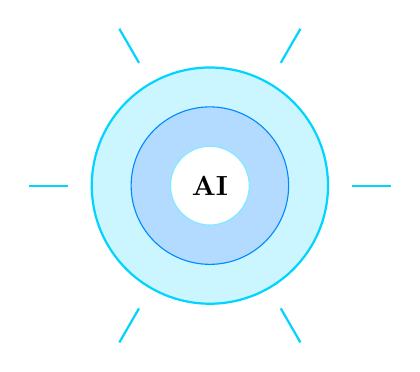
\begin{tikzpicture}
        \draw[fill=phiblue!20, draw=phiblue, thick] (0,0) circle (1.5);
        \draw[fill=phiaccent!30, draw=phiaccent] (0,0) circle (1);
        \draw[fill=white!80, draw=phiblue!50] (0,0) circle (0.5);
        \node at (0,0) {\textbf{AI}};
        \foreach \angle in {0,60,120,180,240,300} {
            \draw[phiblue, thick] (\angle:1.8) -- (\angle:2.3);
        }
    \end{tikzpicture}
    \vfill
}
\author{PHI Agent Development Team}
\date{\today}

\begin{document}

\maketitle
\tableofcontents
\listoffigures
\listoftables

\chapter{Introduction}

\section{Project Overview}

PHI Agent is a modular, production-ready AI personal assistant designed to operate as a comprehensive digital companion with capabilities spanning vision, hearing, speech, long-term memory, smart home control, file management, web interaction, and much more.

The system is built using a \textbf{microservice architecture} with Python-based backend services communicating via Redis Pub/Sub, a React + Three.js frontend for the 3D avatar interface, and a standalone HTML5 equalizer visualization. It supports multiple LLM providers with automatic failover, maintains a Memory Palace with 20 themed rooms using ChromaDB vector storage, and exposes \textbf{300+ tools} across 40+ categories through a LangChain-inspired ReAct (Reasoning + Acting) agent loop with multi-agent orchestration capabilities.

\section{Key Features}

\begin{itemize}[leftmargin=*]
    \item \textbf{Multi-LLM Support:} OpenAI GPT-4, Anthropic Claude, DeepSeek, OpenRouter, local models (Ollama/llama.cpp) with automatic provider failover
    \item \textbf{Memory Palace:} 20 themed rooms with episodic, semantic, procedural, and spatial memory types stored in ChromaDB
    \item \textbf{300+ Tools:} 40+ categories spanning filesystem, web search, email, calendar, smart home, finance, news, sports, entertainment, code execution, database, shopping, color/emotion detection, face recognition, data manipulation, media processing, text intelligence, security, and more
    \item \textbf{Vision System:} YOLOv8 object detection, face recognition, QR/barcode reading, color detection with named-color mapping, palette generation, real-time emotion detection from face images
    \item \textbf{Hearing System:} Always-on microphone with WebRTC VAD, OpenAI Whisper transcription, wake word detection
    \item \textbf{Speech System:} Multi-engine TTS (ElevenLabs, Coqui, gTTS), emotional speech with 8 emotions, viseme/lip-sync generation
    \item \textbf{3D Equalizer:} Three.js circular audio visualizer with 72 radial bars, 5 EQ bands, beat detection, ADSR envelope, bloom post-processing
    \item \textbf{React Frontend:} Three.js 3D avatar, real-time chat, camera feed, audio visualizer, emotion controls
    \item \textbf{Shopping Assistant:} Product search, category browsing, price comparison, policy search, order tracking with SQLite + FAISS vector store
    \item \textbf{Email Agent:} Full email management (search, send, draft, reply, forward, archive, trash), calendar management with HITL (Human-in-the-Loop) approval pattern
    \item \textbf{Understand-Anything Integration:} Interactive knowledge graph generation for any codebase, multi-agent pipeline with tree-sitter + LLM hybrid analysis, guided codebase tours, diff impact analysis
    \item \textbf{Docker Deployment:} 8-container microservice stack with persistent volumes and health checks
\end{itemize}

\section{Technology Stack}

\begin{table}[H]
\centering
\begin{tabularx}{\textwidth}{|l|X|}
\hline
\rowcolor{phiblue!20}
\textbf{Layer} & \textbf{Technologies} \\
\hline
Backend Framework & Python 3.12, FastAPI, Uvicorn \\
\hline
Agent Framework & LangChain-inspired ReAct loop with custom ToolRegistry, multi-agent orchestration, subagent spawning \\
\hline
LLM Providers & OpenAI GPT-4, Anthropic Claude, DeepSeek, OpenRouter, Ollama, llama.cpp \\
\hline
Vector Database & ChromaDB with sentence-transformers embeddings, FAISS for product/policy search \\
\hline
Message Broker & Redis 7 (async Pub/Sub with auto-reconnect) \\
\hline
Object Detection & YOLOv8 nano, OpenCV Haar Cascade \\
\hline
Face Recognition & face\_recognition library, OpenCV, DeepFace (emotion, age, gender, race) \\
\hline
Color Detection & K-means clustering, named-color mapping (24+ colors), KNN, Color Thief algorithm \\
\hline
Speech-to-Text & OpenAI Whisper (local tiny model or API) \\
\hline
Voice Activity Detection & WebRTC VAD \\
\hline
Text-to-Speech & ElevenLabs API, Coqui TTS, gTTS \\
\hline
Frontend & React 18, Three.js 0.150.0, react-three-fiber \\
\hline
Equalizer & Three.js (standalone HTML with importmap), EffectComposer, UnrealBloomPass \\
\hline
Database & SQLite, PostgreSQL, MySQL (via action tools); SQLite for product/email stores \\
\hline
Smart Home & MQTT, Home Assistant integration \\
\hline
Semantic Routing & TF-IDF vectorizer for query classification (shopping vs. general) \\
\hline
Knowledge Graphs & Tree-sitter + LLM hybrid, multi-agent pipeline, interactive dashboard \\
\hline
Containerization & Docker, Docker Compose \\
\hline
Testing & pytest, pytest-asyncio, httpx, pytest-cov \\
\hline
\end{tabularx}
\caption{Technology Stack}
\end{table}

\chapter{System Architecture}

\section{High-Level Architecture}

The system follows a microservice architecture pattern where each major capability is isolated in its own service, all connected through Redis Pub/Sub for asynchronous communication. The Orchestrator acts as the central brain, routing requests between services and managing the agent's reasoning loop.

\begin{figure}[H]
\centering
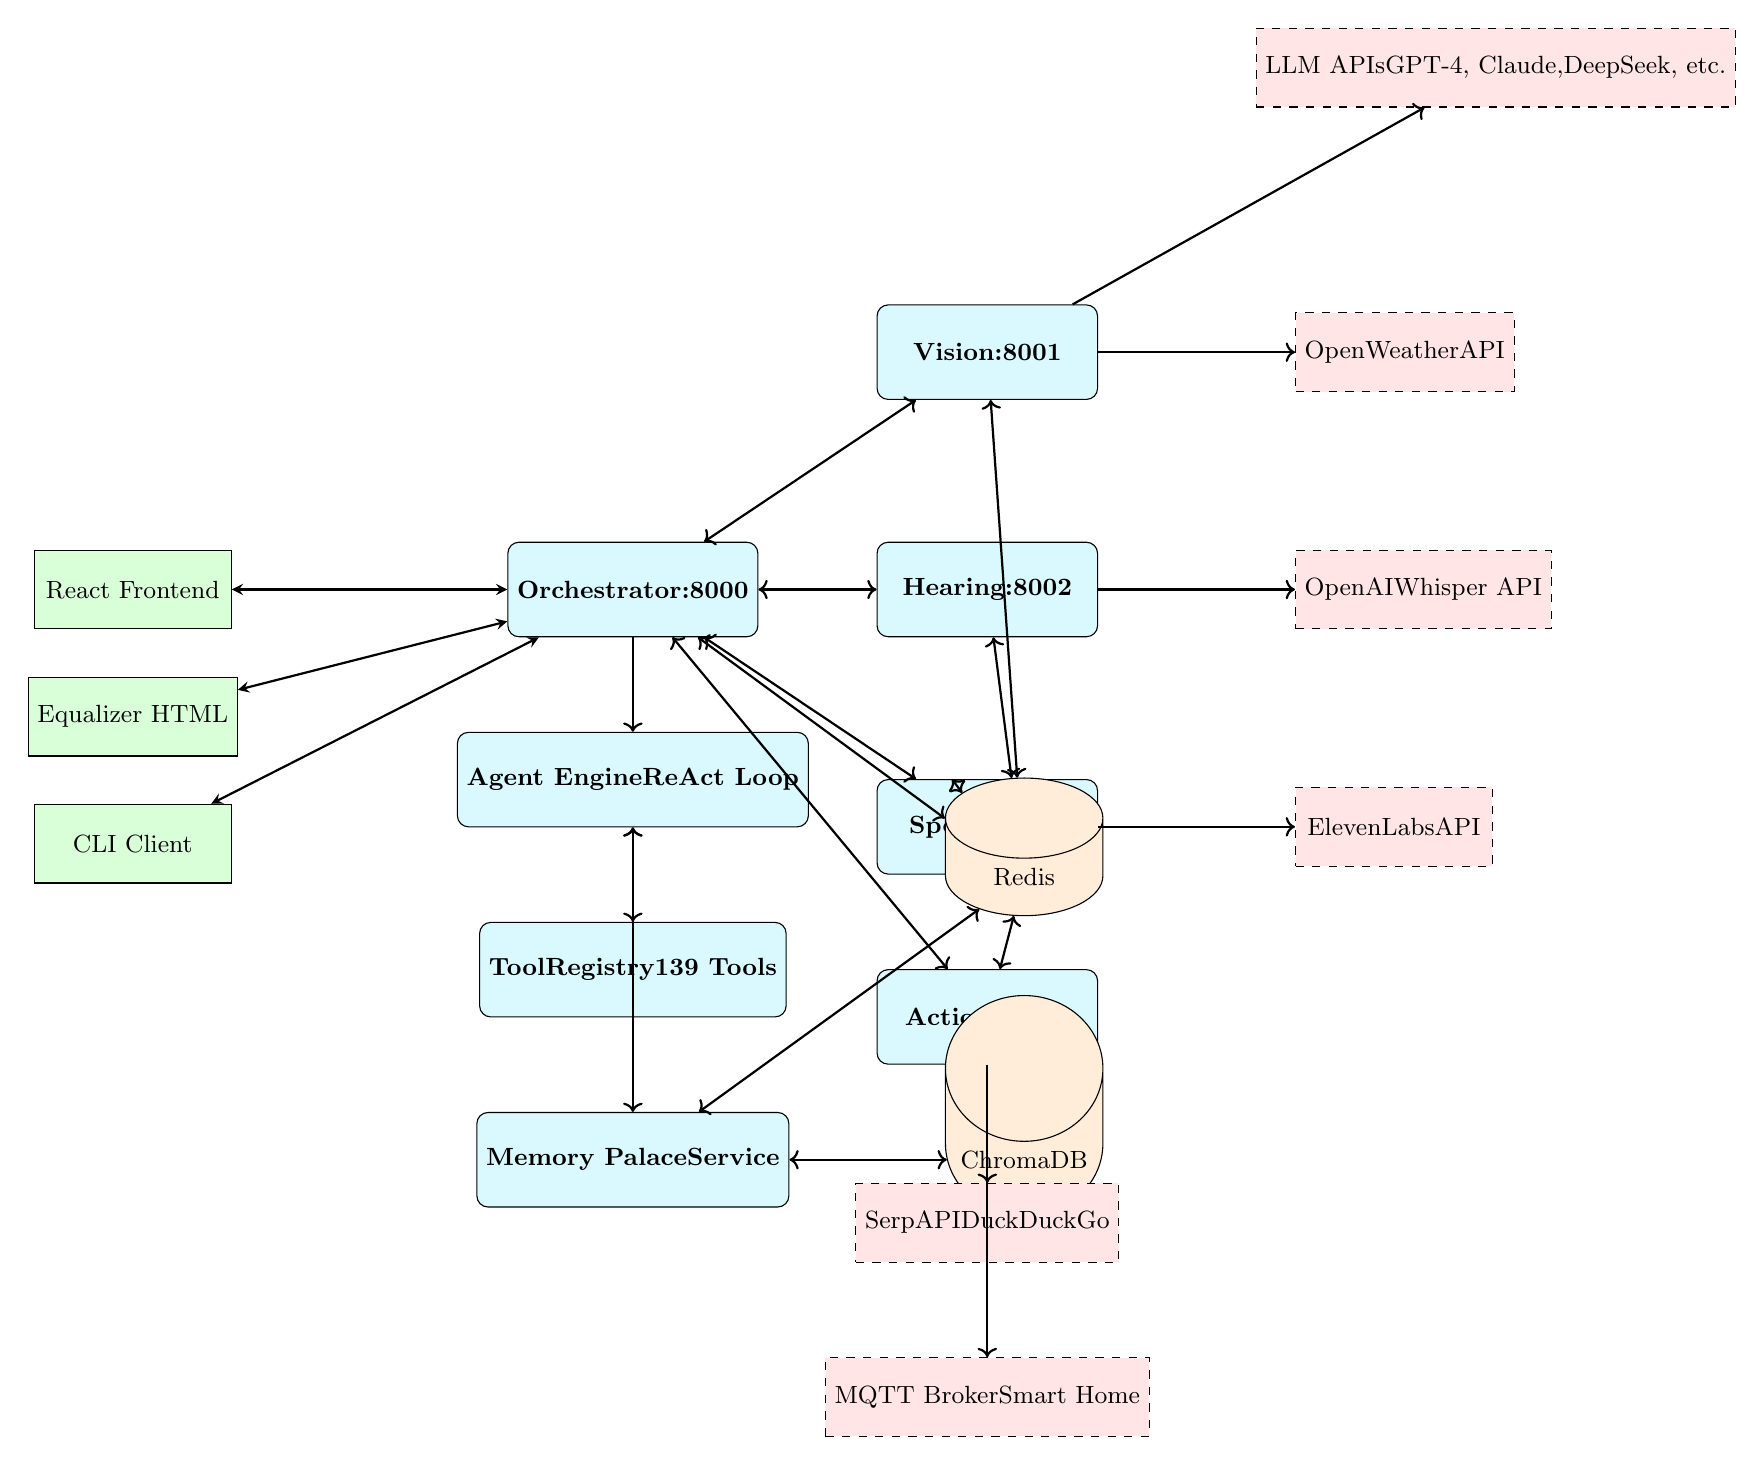
\begin{tikzpicture}[
    node distance=1.8cm,
    service/.style={rectangle, rounded corners, minimum width=2.8cm, minimum height=1.2cm, text centered, draw=black, fill=phiblue!15, font=\small\bfseries},
    db/.style={cylinder, shape border rotate=90, minimum width=2cm, minimum height=1cm, draw=black, fill=orange!15, font=\small},
    client/.style={rectangle, minimum width=2.5cm, minimum height=1cm, text centered, draw=black, fill=green!15, font=\small},
    external/.style={rectangle, dashed, minimum width=2.5cm, minimum height=1cm, text centered, draw=black, fill=red!10, font=\small},
    arrow/.style={thick, ->, >=stealth},
    doublearrow/.style={thick, <->, >=stealth}
]

    % Frontend clients
    \node[client] (react) {React Frontend};
    \node[client, below=0.6cm of react] (eq) {Equalizer HTML};
    \node[client, below=0.6cm of eq] (cli) {CLI Client};
    \coordinate[left=1cm of react] (clients);

    % Orchestrator
    \node[service, right=3.5cm of react] (orch) {Orchestrator\\:8000};
    \node[service, below=1.2cm of orch] (agent) {Agent Engine\\ReAct Loop};
    \node[service, below=1.2cm of agent] (tools) {ToolRegistry\\139 Tools};

    % Support services
    \node[service, above right=1.8cm and 1.5cm of orch] (vision) {Vision\\:8001};
    \node[service, right=1.5cm of orch] (hearing) {Hearing\\:8002};
    \node[service, below right=1.8cm and 1.5cm of orch] (speech) {Speech\\:8003};
    \node[service, below=1.2cm of speech] (action) {Actions\\:8004};

    % Memory & Data
    \node[service, below=1.2cm of tools] (memory) {Memory Palace\\Service};
    \node[db, right=2cm of memory] (chroma) {ChromaDB};
    \node[db, above=1cm of chroma] (redis) {Redis};

    % External APIs
    \node[external, above right=2.5cm and 2cm of vision] (llm) {LLM APIs\\GPT-4, Claude,\\DeepSeek, etc.};
    \node[external, right=2.5cm of vision] (openweather) {OpenWeather\\API};
    \node[external, right=2.5cm of hearing] (openai) {OpenAI\\Whisper API};
    \node[external, right=2.5cm of speech] (eleven) {ElevenLabs\\API};
    \node[external, below=1.5cm of action] (serp) {SerpAPI\\DuckDuckGo};
    \node[external, below=1.2cm of serp] (mqtt) {MQTT Broker\\Smart Home};

    % Connections
    \draw[doublearrow] (react) -- (orch);
    \draw[doublearrow] (eq) -- (orch);
    \draw[doublearrow] (cli) -- (orch);
    \draw[->, thick] (orch) -- (agent);
    \draw[<->, thick] (agent) -- (tools);
    \draw[<->, thick] (agent) -- (memory);
    \draw[<->, thick] (orch) -- (vision);
    \draw[<->, thick] (orch) -- (hearing);
    \draw[<->, thick] (orch) -- (speech);
    \draw[<->, thick] (orch) -- (action);
    \draw[<->, thick] (memory) -- (chroma);
    \draw[<->, thick] (memory) -- (redis);
    \draw[<->, thick] (orch) -- (redis);
    \draw[<->, thick] (vision) -- (redis);
    \draw[<->, thick] (hearing) -- (redis);
    \draw[<->, thick] (speech) -- (redis);
    \draw[<->, thick] (action) -- (redis);
    \draw[->, thick] (vision) -- (llm);
    \draw[->, thick] (vision) -- (openweather);
    \draw[->, thick] (hearing) -- (openai);
    \draw[->, thick] (speech) -- (eleven);
    \draw[->, thick] (action) -- (serp);
    \draw[->, thick] (action) -- (mqtt);

\end{tikzpicture}
\caption{High-Level System Architecture}
\label{fig:architecture}
\end{figure}

\section{Service Communication Architecture}

All services communicate through Redis Pub/Sub using a request/response pattern. The \texttt{RedisPubSub} class in \texttt{backend/shared/redis\_client.py} provides automatic reconnection, channel-based message routing, and typed RPC stubs defined in \texttt{grpc\_stubs.py}.

\begin{figure}[H]
\centering
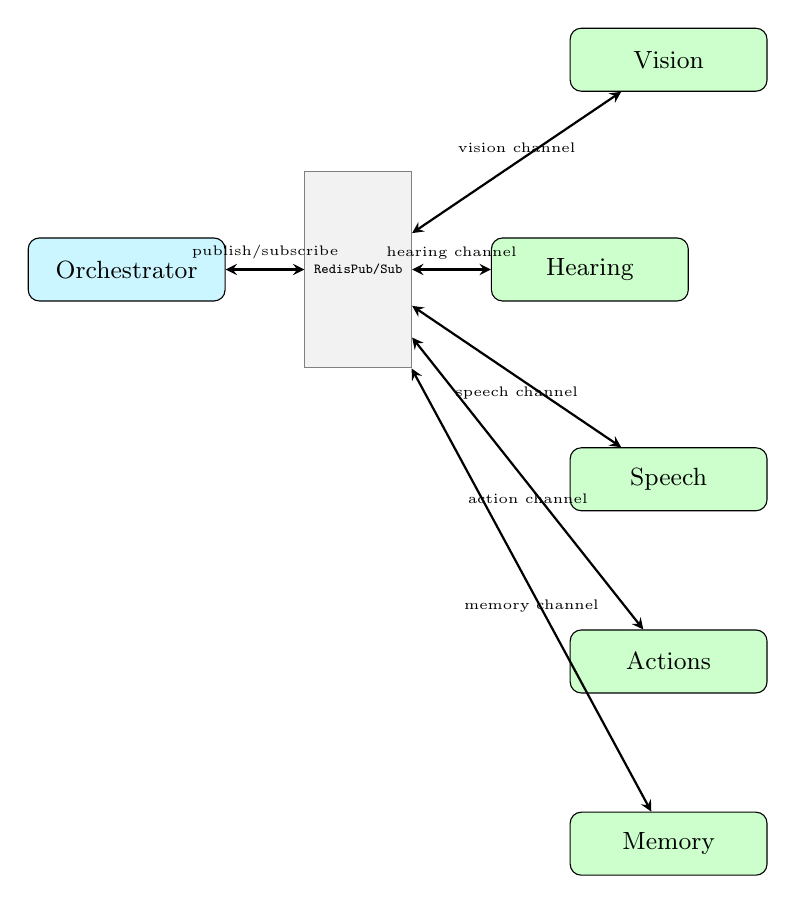
\begin{tikzpicture}[
    node distance=1.5cm,
    block/.style={rectangle, rounded corners, minimum width=2.5cm, minimum height=0.8cm, text centered, draw=black, font=\small},
    channel/.style={rectangle, minimum width=0.6cm, minimum height=2.5cm, draw=black!50, fill=gray!10, font=\tiny\ttfamily},
    arrow/.style={thick, ->, >=stealth},
    doublearrow/.style={thick, <->, >=stealth}
]

    \node[block, fill=phiblue!20] (orch) {Orchestrator};
    \node[channel, right=1cm of orch] (redis) {Redis\\Pub/Sub};
    \node[block, above right=1cm and 2cm of redis, fill=green!20] (vis) {Vision};
    \node[block, right=1cm of redis, fill=green!20] (hear) {Hearing};
    \node[block, below right=1cm and 2cm of redis, fill=green!20] (sp) {Speech};
    \node[block, below=1.5cm of sp, fill=green!20] (act) {Actions};
    \node[block, below=1.5cm of act, fill=green!20] (mem) {Memory};

    \draw[doublearrow] (orch) -- node[above, font=\tiny] {publish/subscribe} (redis);
    \draw[doublearrow] (vis) -- node[above, font=\tiny] {vision channel} (redis);
    \draw[doublearrow] (hear) -- node[above, font=\tiny] {hearing channel} (redis);
    \draw[doublearrow] (sp) -- node[below, font=\tiny] {speech channel} (redis);
    \draw[doublearrow] (act) -- node[below, font=\tiny] {action channel} (redis);
    \draw[doublearrow] (mem) -- node[below, font=\tiny] {memory channel} (redis);

\end{tikzpicture}
\caption{Redis Pub/Sub Communication Pattern}
\label{fig:redis-comm}
\end{figure}

\section{Deployment Architecture}

The system is containerized using Docker Compose with 8 services, persistent volumes for Redis and ChromaDB, and a shared bridge network.

\begin{figure}[H]
\centering
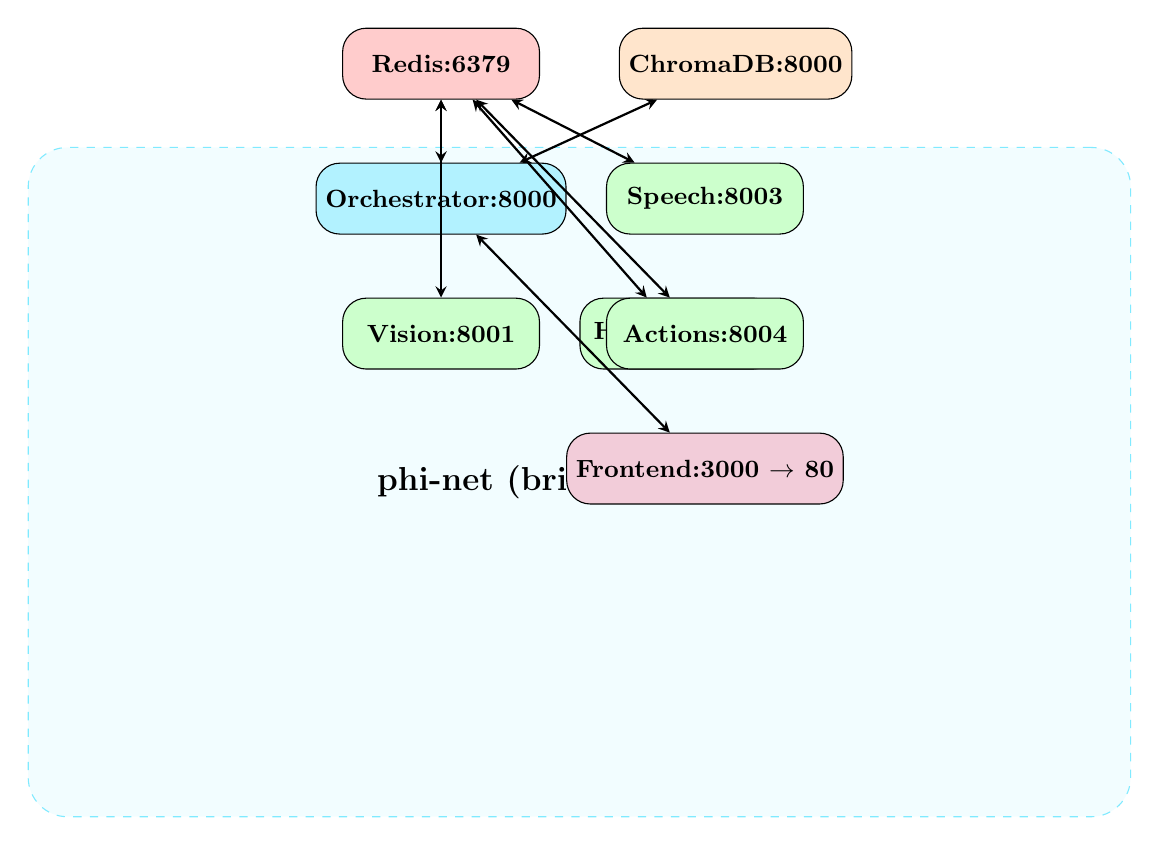
\begin{tikzpicture}[
    node distance=1.2cm,
    container/.style={rectangle, rounded corners=3mm, minimum width=2.5cm, minimum height=0.9cm, text centered, draw=black, font=\small\bfseries},
    net/.style={rectangle, rounded corners=5mm, minimum width=14cm, minimum height=8.5cm, draw=phiblue!50, fill=phiblue!5, dashed, font=\large},
    arrow/.style={thick, <->, >=stealth}
]

    \node[net] (net) {\textbf{phi-net (bridge network)}};

    \node[container, fill=red!20, above left=0.6cm and 0.5cm of net.north] (redis) {Redis\\:6379};
    \node[container, fill=orange!20, above right=0.6cm and 0.5cm of net.north] (chroma) {ChromaDB\\:8000};
    \node[container, fill=phiblue!30, below=0.8cm of redis] (orch) {Orchestrator\\:8000};
    \node[container, fill=green!20, below=0.8cm of orch] (vision) {Vision\\:8001};
    \node[container, fill=green!20, right=0.5cm of vision] (hearing) {Hearing\\:8002};
    \node[container, fill=green!20, right=0.5cm of orch] (speech) {Speech\\:8003};
    \node[container, fill=green!20, below=0.8cm of speech] (action) {Actions\\:8004};
    \node[container, fill=purple!20, below=0.8cm of action] (frontend) {Frontend\\:3000 $\rightarrow$ 80};

    \draw[arrow] (orch) -- (redis);
    \draw[arrow] (orch) -- (chroma);
    \draw[arrow] (vision) -- (redis);
    \draw[arrow] (hearing) -- (redis);
    \draw[arrow] (speech) -- (redis);
    \draw[arrow] (action) -- (redis);
    \draw[arrow] (frontend) -- (orch);

\end{tikzpicture}
\caption{Docker Compose Deployment Architecture}
\label{fig:deployment}
\end{figure}

\chapter{Core Components}

\section{Orchestrator Service}

The Orchestrator is the central brain of PHI Agent, implemented as a FastAPI application in \texttt{backend/orchestrator/main.py}. It manages WebSocket connections, routes chat requests to the agent, coordinates between microservices, and handles session management.

\subsection{API Endpoints}

\begin{longtable}{|l|l|p{6cm}|l|}
\hline
\rowcolor{phiblue!20}
\textbf{Method} & \textbf{Endpoint} & \textbf{Description} & \textbf{Response Model} \\
\hline
GET & /health & Health check with uptime, session count, memory status & StatusResponse \\
\hline
POST & /chat & Main conversation endpoint & ChatResponse \\
\hline
POST & /chat/stream & SSE streaming chat with token-by-token output & Event Stream \\
\hline
GET & /avatar/expression & Get avatar blend shapes for emotion & ExpressionResponse \\
\hline
POST & /vision/scene & Scene understanding from camera image & SceneResponse \\
\hline
POST & /session & Create a new session & SessionInfo \\
\hline
GET & /session/\{session\_id\} & Get session information & SessionInfo \\
\hline
GET & /status & System status with tool listing & StatusResponse \\
\hline
WS & /ws & Bidirectional WebSocket (chat, audio, image, commands) & WebSocketMessage \\
\hline
\end{longtable}
\caption{Orchestrator API Endpoints}

\subsection{WebSocket Protocol}

The WebSocket at \texttt{/ws} supports multiple message types for bidirectional communication:

\begin{table}[H]
\centering
\begin{tabularx}{\textwidth}{|l|X|}
\hline
\rowcolor{phiblue!20}
\textbf{Message Type} & \textbf{Payload} \\
\hline
chat & \{ text: string, session\_id: string, emotion?: string \} \\
\hline
audio & \{ audio: base64-string, session\_id: string \} \\
\hline
image & \{ image: base64-string, session\_id: string \} \\
\hline
command & \{ action: string, params?: object \} \\
\hline
mode & \{ mode: "listening" | "thinking" | "speaking" \} \\
\hline
emotion & \{ emotion: string \} \\
\hline
visemes & \{ frames: array \} \\
\hline
ping/pong & \{ \} \\
\hline
\end{tabularx}
\caption{WebSocket Message Types}
\end{table}

\subsection{Session Management}

Sessions are stored in-memory as a dictionary mapping session IDs to session objects:

\begin{table}[H]
\centering
\rowcolors{2}{gray!10}{white}
\begin{tabularx}{\textwidth}{|l|X|}
\hline
\rowcolor{phiblue!20}
\textbf{Field} & \textbf{Description} \\
\hline
created\_at & Session creation timestamp \\
\hline
last\_active & Timestamp of last interaction \\
\hline
message\_count & Total messages in session \\
\hline
emotion & Current emotional state \\
\hline
user\_name & Identified user name \\
\hline
\end{tabularx}
\caption{Session Data Fields}
\end{table}

\section{Agent Engine}

\subsection{The ReAct Loop}

The agent uses a Reasoning + Acting (ReAct) loop pattern. Each iteration follows: \textbf{Thought $\rightarrow$ Action $\rightarrow$ Observation $\rightarrow$ Response}.

\begin{figure}[H]
\centering
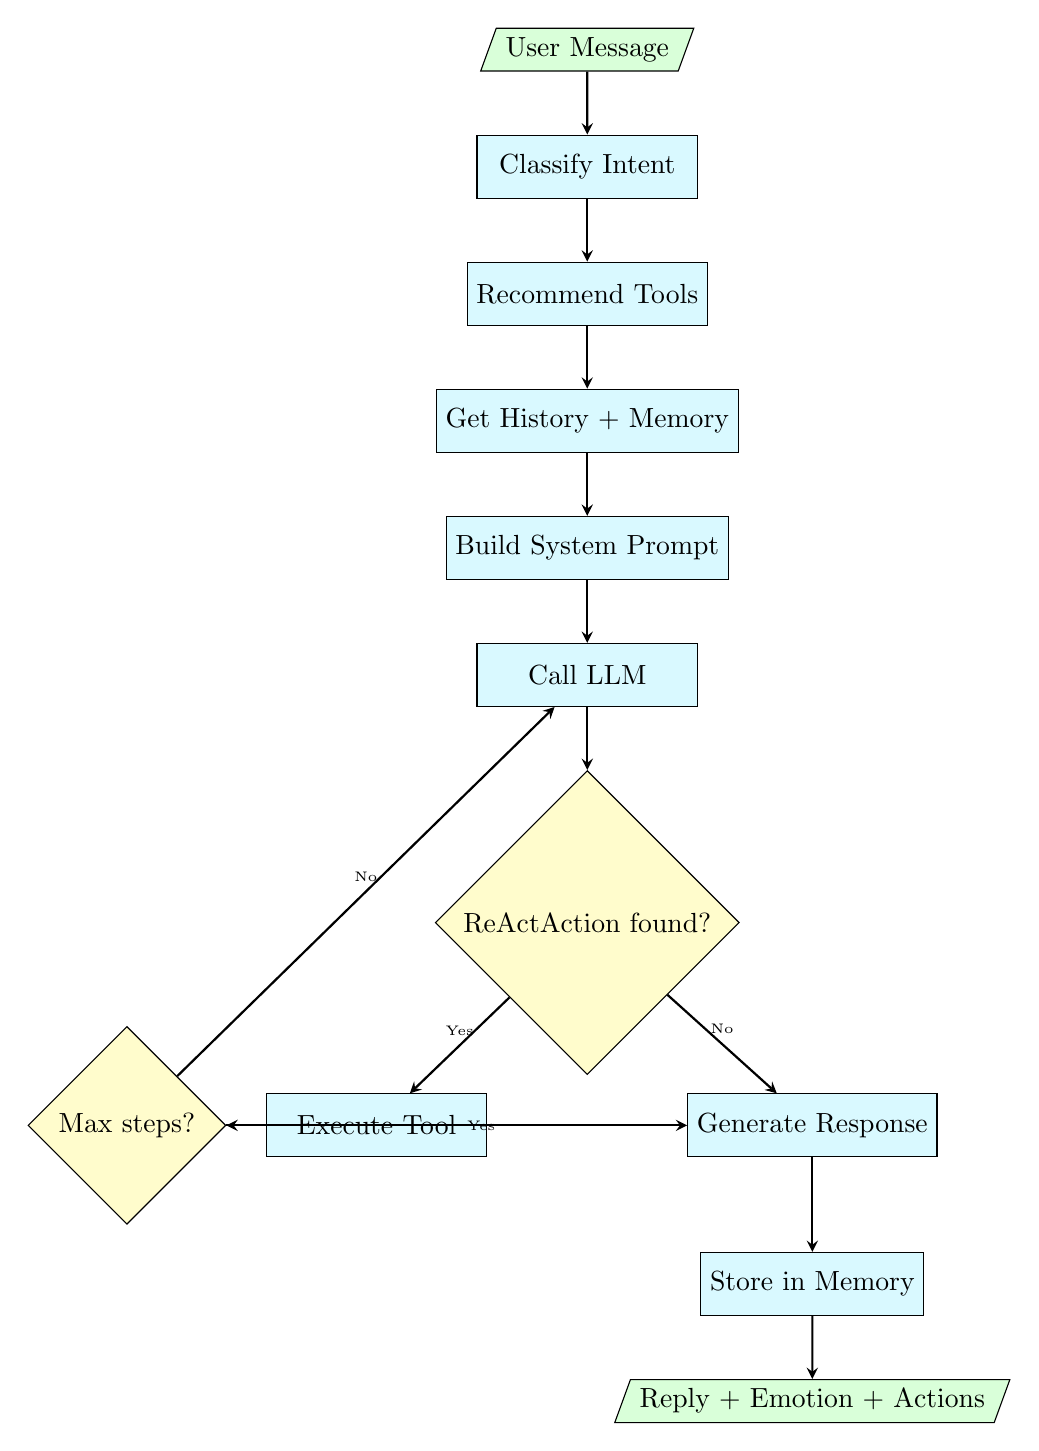
\begin{tikzpicture}[
    node distance=1.2cm,
    startstop/.style={rectangle, rounded corners, minimum width=2.5cm, minimum height=0.8cm, text centered, draw=black, fill=red!20},
    process/.style={rectangle, minimum width=2.8cm, minimum height=0.8cm, text centered, draw=black, fill=phiblue!15},
    decision/.style={diamond, minimum width=1.8cm, minimum height=1.2cm, text centered, draw=black, fill=yellow!20},
    io/.style={trapezium, trapezium left angle=70, trapezium right angle=110, minimum width=2cm, text centered, draw=black, fill=green!15},
    arrow/.style={thick, ->, >=stealth}
]

    \node[io] (input) {User Message};
    \node[process, below=0.8cm of input] (classify) {Classify Intent};
    \node[process, below=0.8cm of classify] (tools) {Recommend Tools};
    \node[process, below=0.8cm of tools] (history) {Get History + Memory};
    \node[process, below=0.8cm of history] (system) {Build System Prompt};
    \node[process, below=0.8cm of system] (llm) {Call LLM};
    \node[decision, below=0.8cm of llm] (react) {ReAct\\Action found?};
    \node[process, below left=1.2cm and 0.3cm of react] (execute) {Execute Tool};
    \node[process, below right=1.2cm and 0.3cm of react] (respond) {Generate Response};
    \node[process, below=1.2cm of respond] (store) {Store in Memory};
    \node[io, below=0.8cm of store] (output) {Reply + Emotion + Actions};
    \node[decision, left=0.5cm of execute] (loop) {Max steps?};

    \draw[arrow] (input) -- (classify);
    \draw[arrow] (classify) -- (tools);
    \draw[arrow] (tools) -- (history);
    \draw[arrow] (history) -- (system);
    \draw[arrow] (system) -- (llm);
    \draw[arrow] (llm) -- (react);
    \draw[arrow] (react) -- node[above, font=\tiny] {Yes} (execute);
    \draw[arrow] (react) -- node[above, font=\tiny] {No} (respond);
    \draw[arrow] (execute) -- (loop);
    \draw[arrow] (loop) -- node[above, font=\tiny] {No} (llm);
    \draw[arrow] (loop) -- node[right, font=\tiny] {Yes} (respond);
    \draw[arrow] (respond) -- (store);
    \draw[arrow] (store) -- (output);

\end{tikzpicture}
\caption{Agent ReAct Processing Loop}
\label{fig:react-loop}
\end{figure}

\subsection{ToolRegistry}

The \texttt{ToolRegistry} class (in \texttt{backend/orchestrator/agent.py}) manages all 300+ tools. Each tool is registered as a \texttt{Tool} dataclass with the following fields:

\begin{table}[H]
\centering
\rowcolors{2}{gray!10}{white}
\begin{tabularx}{\textwidth}{|l|X|}
\hline
\rowcolor{phiblue!20}
\textbf{Field} & \textbf{Description} \\
\hline
name & Unique tool identifier \\
\hline
description & Natural-language description for LLM selection \\
\hline
parameters & JSON Schema describing accepted parameters \\
\hline
handler & Async callable that executes the tool \\
\hline
requires\_confirmation & Whether HITL confirmation is needed \\
\hline
category & Logical category grouping (vision, data, finance, etc.) \\
\hline
\end{tabularx}
\caption{Tool Dataclass Fields}
\end{table}

\subsection{Tool Categories}

The 300+ tools are organized into the following categories:

\begin{table}[H]
\centering
\rowcolors{2}{gray!10}{white}
\begin{tabularx}{\textwidth}{|l|r|X|}
\hline
\rowcolor{phiblue!20}
\textbf{Category} & \textbf{Count} & \textbf{Example Tools} \\
\hline
utility & 15 & get\_time, get\_world\_time, random\_number, random\_choice, color\_convert, math\_calculate, query\_yesno \\
\hline
information & 5 & search\_web, get\_weather, search\_academic, scrape\_page, firecrawl\_scrape \\
\hline
communication & 5 & send\_email, read\_inbox, search\_emails, slack\_send, discord\_send \\
\hline
productivity & 8 & create\_calendar\_event, set\_reminder, get\_upcoming\_events, schedule\_reminder, schedule\_at, list\_scheduled\_tasks, cancel\_task, notion\_create \\
\hline
smart\_home & 6 & control\_light, set\_temperature, set\_light\_scene, set\_humidity, lock\_door, get\_energy\_usage \\
\hline
system & 15+ & mouse\_move, mouse\_click, keyboard\_type, keyboard\_hotkey, window\_manage, screenshot, system\_settings\_control, multi\_monitor, startup\_program, macro\_record, macro\_run, orchestrate\_sequence \\
\hline
memory & 5 & remember, recall, summarize\_memory, remember\_topic, remember\_preference \\
\hline
vision & 12+ & detect\_colors, analyze\_scene, extract\_dominant\_colors, color\_name\_from\_rgb/hex, color\_palette\_generate, color\_analyze\_image\_url/local, detect\_emotion\_face, detect\_faces\_image, analyze\_face\_attributes, compare\_faces \\
\hline
avatar & 1 & get\_avatar\_expression \\
\hline
filesystem & 20+ & read\_file, write\_file, list\_files, delete\_file, search\_files, file\_hash, file\_diff, file\_compress, file\_type\_detect, obsidian\_* (5 tools) \\
\hline
data & 35+ & read\_csv, query\_csv, read\_excel, read\_json, query\_json, str\_reverse, str\_upper, str\_split, str\_join, list\_shuffle, list\_unique, list\_flatten, dict\_merge, json\_flatten, stat\_mean, stat\_median, stat\_correlation \\
\hline
development & 10+ & run\_python, run\_javascript, git\_* (6 tools), generate\_code, generate\_git\_commit, generate\_dockerfile \\
\hline
finance & 10+ & get\_stock\_price, get\_market\_indices, get\_company\_info, get\_stock\_historical, get\_top\_movers, convert\_currency, get\_exchange\_rates, polygon\_stock\_price, stripe\_* \\
\hline
news & 4 & get\_news, get\_stock\_news, scrape\_hacker\_news, scrape\_news \\
\hline
crypto & 2 & get\_crypto\_price, get\_trending\_crypto \\
\hline
sports & 1 & get\_sports\_scores \\
\hline
entertainment & 6+ & get\_movie\_info, get\_trending\_movies, spotify\_*, recommend\_movie, get\_music\_recommendations, get\_daily\_quote \\
\hline
food & 2 & get\_nutrition, search\_recipes \\
\hline
reference & 6+ & define\_word, get\_synonyms, get\_holidays, get\_ip\_info, search\_books, scrape\_wikipedia \\
\hline
fun & 4 & get\_joke, get\_quote, get\_random\_fact, desktop\_pet\_* \\
\hline
science & 3 & get\_nasa\_apod, get\_iss\_location, get\_people\_in\_space \\
\hline
music & 2 & get\_top\_songs, spotify\_search\_and\_play \\
\hline
web & 8+ & scrape\_url, web\_search\_scrape, scrape\_github\_trending, compare\_prices, scrape\_product, scrape\_jobs, scrape\_translate, scrape\_facts \\
\hline
visualization & 25+ & plot\_line\_chart, plot\_bar\_chart, plot\_pie\_chart, plot\_stock\_chart, visualize\_data, plot\_scatter, plot\_histogram, plot\_heatmap, plot\_correlation, plot\_radar, plot\_box, plot\_violin, plot\_3d\_surface, plot\_waterfall, plot\_candlestick, plot\_network\_graph, plot\_sunburst \\
\hline
automation & 3 & run\_automation, zapier\_trigger, webhook\_* \\
\hline
calendar & 8+ & list\_calendar\_events, find\_meeting\_slots, calendar\_create, calendar\_update, calendar\_delete, calendar\_find\_slots \\
\hline
shopping & 12 & product\_search\_db, product\_get\_details, product\_list\_categories, policy\_search, get\_product\_recommendations, check\_store\_policy, track\_order, shopping\_route\_query, compare\_prices \\
\hline
email & 15+ & email\_search, email\_list\_inbox, email\_get\_message, email\_send, email\_draft, email\_reply, email\_mark\_read, email\_star, email\_archive, email\_trash, email\_forward, email\_search\_by\_sender, email\_get\_unread\_count, email\_get\_attachment \\
\hline
health & 4 & log\_workout, log\_meal, start\_meditation, fitbit\_get\_steps \\
\hline
travel & 3 & get\_flight\_info, get\_restaurant\_recommendations, travel\_agent\_* \\
\hline
security & 10+ & generate\_password, check\_password\_strength, auth\_create\_token, auth\_verify\_token, permission\_check, sanitize\_input, audit\_log, session\_create \\
\hline
notifications & 3 & send\_notification, schedule\_notification, daily\_briefing \\
\hline
learning & 3 & generate\_flashcard, explain\_concept, detect\_language \\
\hline
creative & 12+ & generate\_image, generate\_writing\_prompt, generate\_color\_palette, audio\_trim, audio\_concatenate, audio\_effects\_apply, audio\_format\_convert, audio\_noise\_reduce, holographic\_ui\_render \\
\hline
social & 2 & get\_upcoming\_birthdays, telegram\_send\_message \\
\hline
ai\_capabilities & 6+ & debate\_topic, spawn\_agent, list\_agents, multi\_agent\_collaborate, swarm\_*, predictive\_analyze \\
\hline
personality & 10+ & create\_persona, delete\_persona, communication\_style\_report, digital\_twin\_learn, digital\_twin\_mimic, emotion\_companion\_* \\
\hline
audio & 10+ & audio\_trim, audio\_concatenate, audio\_split\_by\_silence, audio\_effects\_apply, audio\_format\_convert, audio\_noise\_reduce, audio\_mix\_tracks \\
\hline
media & 30+ & format\_convert, csv\_*, geo\_*, time\_*, color\_palette (analogous/triadic/complementary), file\_copy/move/rename, http\_get/post, url\_encode/decode, base64\_encode/decode, json\_prettify/minify, html\_escape, slugify \\
\hline
vision (advanced) & 12 & extract\_dominant\_colors, color\_name\_from\_rgb, color\_name\_from\_hex, color\_palette\_generate, color\_analyze\_image\_url, color\_analyze\_local\_image, detect\_emotion\_face, detect\_emotion\_text, detect\_faces\_image, analyze\_face\_attributes, compare\_faces, analyze\_emotion\_realtime \\
\hline
\end{tabularx}
\caption{All Tool Categories}
\end{table}

\subsection{Intent Classification}

The agent classifies user messages into 21 intent patterns using keyword matching in \texttt{\_classify\_intent()}:

\begin{table}[H]
\centering
\begin{tabularx}{\textwidth}{|l|X|}
\hline
\rowcolor{phiblue!20}
\textbf{Intent} & \textbf{Keywords/Patterns} \\
\hline
greeting & hello, hi, hey, good morning, good evening, yo \\
\hline
farewell & goodbye, bye, see you, good night, talk later \\
\hline
time\_query & time, date, what day, current time, what's the date \\
\hline
weather\_query & weather, temperature, forecast, rain, sunny \\
\hline
search\_query & search, find, look up, google, research \\
\hline
knowledge\_query & what is, who is, explain, define, tell me about, how does \\
\hline
email\_task & email, send mail, compose, draft, write to \\
\hline
calendar\_task & calendar, event, schedule, appointment, meeting \\
\hline
reminder\_task & remind, reminder, remember to, notify me \\
\hline
file\_task & file, read, write, save, open, create, delete, list, folder, directory \\
\hline
music\_task & play, music, song, spotify, playlist \\
\hline
code\_task & code, program, script, function, algorithm, debug \\
\hline
joke\_request & joke, funny, humor, make me laugh \\
\hline
quote\_request & quote, inspiration, motivate \\
\hline
stock\_query & stock, share price, market, ticker, aapl, tsla \\
\hline
chart\_request & chart, graph, plot, visualize \\
\hline
help\_request & help, what can you do, capabilities, commands \\
\hline
status\_query & status, how are you, what's up, are you there \\
\hline
memory\_query & remember, recall, what do you know about, memories \\
\hline
translation & translate, in spanish, in french, how do you say \\
\hline
debate\_request & debate, argue, discuss, pros and cons, compare viewpoints \\
\hline
general\_conversation & (default -- no specific pattern matched) \\
\hline
\end{tabularx}
\caption{Intent Classification Patterns}
\end{table}

\section{Memory Palace}

\subsection{Memory Types}

The Memory Palace system (\texttt{backend/memory/service.py}) implements a sophisticated long-term memory architecture with four distinct memory types:

\begin{table}[H]
\centering
\begin{tabularx}{\textwidth}{|l|X|}
\hline
\rowcolor{phiblue!20}
\textbf{Memory Type} & \textbf{Description} \\
\hline
Episodic & Personal experiences and events (e.g., "User asked about weather yesterday at 3pm") \\
\hline
Semantic & Facts and general knowledge (e.g., "User's favorite color is blue") \\
\hline
Procedural & How-to knowledge and processes (e.g., "How the user likes their emails formatted") \\
\hline
Spatial & Spatial and location-based memories (e.g., "Smart light in living room is called 'main'") \\
\hline
\end{tabularx}
\caption{Memory Types}
\end{table}

\subsection{Memory Importance Levels}

Each memory trace has an importance level that affects its retention and retrieval priority:

\begin{table}[H]
\centering
\begin{tabularx}{\textwidth}{|l|X|}
\hline
\rowcolor{phiblue!20}
\textbf{Level} & \textbf{Description} \\
\hline
TRIVIAL & Low-value, easily forgettable (e.g., "User said 'ok'") \\
\hline
LOW & Minor facts or casual mentions \\
\hline
NORMAL & Standard memories (conversation summaries) \\
\hline
HIGH & Important information (user preferences, key facts) \\
\hline
CRITICAL & Essential data (passwords, configurations, critical instructions) \\
\hline
\end{tabularx}
\caption{Memory Importance Levels}
\end{table}

\subsection{The 20 Memory Palace Rooms}

The memory palace consists of 20 themed rooms, each designed for a specific domain of knowledge:

\begin{table}[H]
\centering
\begin{tabularx}{\textwidth}{|l|X|}
\hline
\rowcolor{phiblue!20}
\textbf{Room Name} & \textbf{Description / Topic} \\
\hline
Grand Foyer & First impressions, user identity, core preferences \\
\hline
Library & Books, learning, knowledge, academic interests \\
\hline
Workshop & Projects, development, code, technical skills \\
\hline
Garden & Nature, hobbies, relaxation, personal growth \\
\hline
Kitchen & Food, recipes, nutrition, cooking preferences \\
\hline
Living Room & Social interactions, family, friends, relationships \\
\hline
Study Room & Work, career, productivity, professional goals \\
\hline
Music Room & Music, playlists, instruments, audio preferences \\
\hline
Art Gallery & Visual arts, design, creativity, aesthetic preferences \\
\hline
Home Theater & Movies, TV shows, entertainment preferences \\
\hline
Gym & Fitness, health, exercise routines, wellness goals \\
\hline
Travel Desk & Travel plans, destinations, trips, geography \\
\hline
Command Center & Smart home configuration, devices, automation rules \\
\hline
Vault & Security, passwords, sensitive information (encrypted) \\
\hline
Observatory & Science, space, technology, research interests \\
\hline
Greenhouse & Environment, sustainability, climate preferences \\
\hline
Archive & Historical data, past conversations, long-term trends \\
\hline
Workshop II & Side projects, experiments, creative endeavors \\
\hline
Gaming Room & Games, sports, competitive interests \\
\hline
Zen Garden & Meditation, mindfulness, emotional state, mood patterns \\
\hline
\end{tabularx}
\caption{Memory Palace Rooms}
\end{table}

\subsection{Memory Flow Diagram}

\begin{figure}[H]
\centering
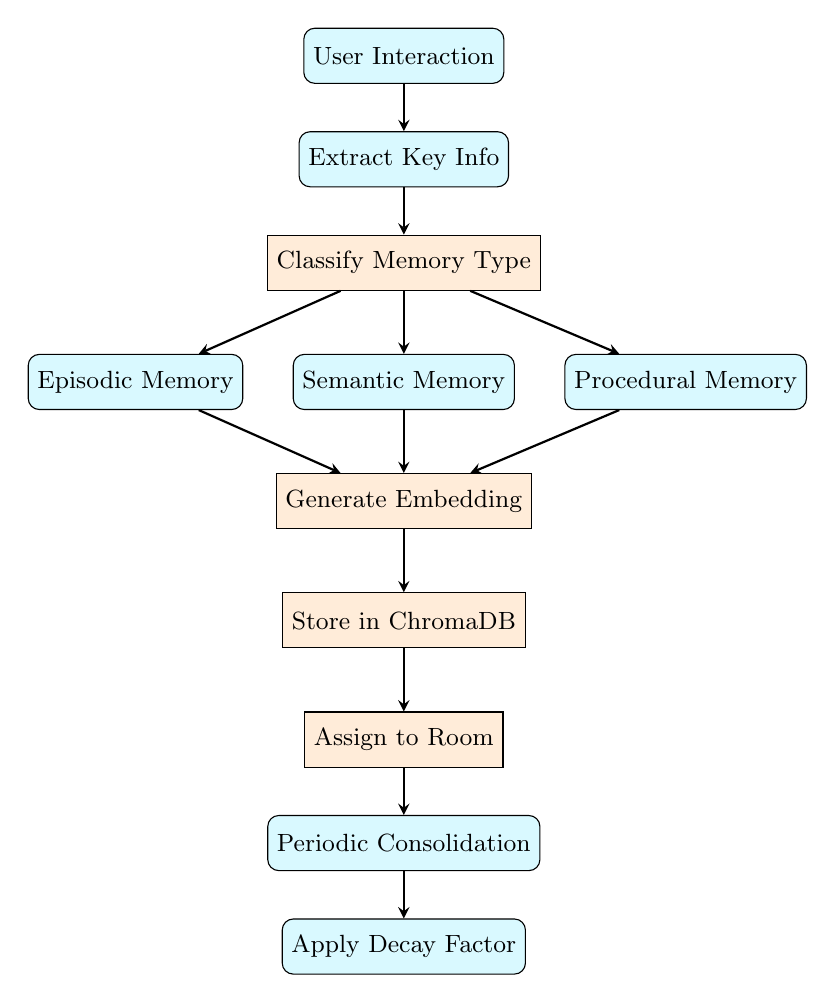
\begin{tikzpicture}[
    node distance=1.2cm,
    process/.style={rectangle, rounded corners, minimum width=2.5cm, minimum height=0.7cm, text centered, draw=black, fill=phiblue!15, font=\small},
    store/.style={rectangle, minimum width=2.5cm, minimum height=0.7cm, text centered, draw=black, fill=orange!15, font=\small},
    arrow/.style={thick, ->, >=stealth}
]

    \node[process] (input) {User Interaction};
    \node[process, below=0.6cm of input] (extract) {Extract Key Info};
    \node[store, below=0.6cm of extract] (classify) {Classify Memory Type};
    \node[process, below left=0.8cm and 0.3cm of classify] (episodic) {Episodic Memory};
    \node[process, below=0.8cm of classify] (semantic) {Semantic Memory};
    \node[process, below right=0.8cm and 0.3cm of classify] (procedural) {Procedural Memory};
    \node[store, below=0.8cm of semantic] (embed) {Generate Embedding};
    \node[store, below=0.8cm of embed] (chroma) {Store in ChromaDB};
    \node[store, below=0.8cm of chroma] (assign) {Assign to Room};
    \node[process, below=0.6cm of assign] (summarize) {Periodic Consolidation};
    \node[process, below=0.6cm of summarize] (decay) {Apply Decay Factor};

    \draw[arrow] (input) -- (extract);
    \draw[arrow] (extract) -- (classify);
    \draw[arrow] (classify) -- (episodic);
    \draw[arrow] (classify) -- (semantic);
    \draw[arrow] (classify) -- (procedural);
    \draw[arrow] (episodic) -- (embed);
    \draw[arrow] (semantic) -- (embed);
    \draw[arrow] (procedural) -- (embed);
    \draw[arrow] (embed) -- (chroma);
    \draw[arrow] (chroma) -- (assign);
    \draw[arrow] (assign) -- (summarize);
    \draw[arrow] (summarize) -- (decay);

\end{tikzpicture}
\caption{Memory Storage Flow}
\label{fig:memory-flow}
\end{figure}

\section{LLM Client}

\subsection{Provider Architecture}

The \texttt{LLMClient} class (\texttt{backend/shared/llm\_client.py}) provides a unified interface to multiple LLM providers with automatic failover:

\begin{figure}[H]
\centering
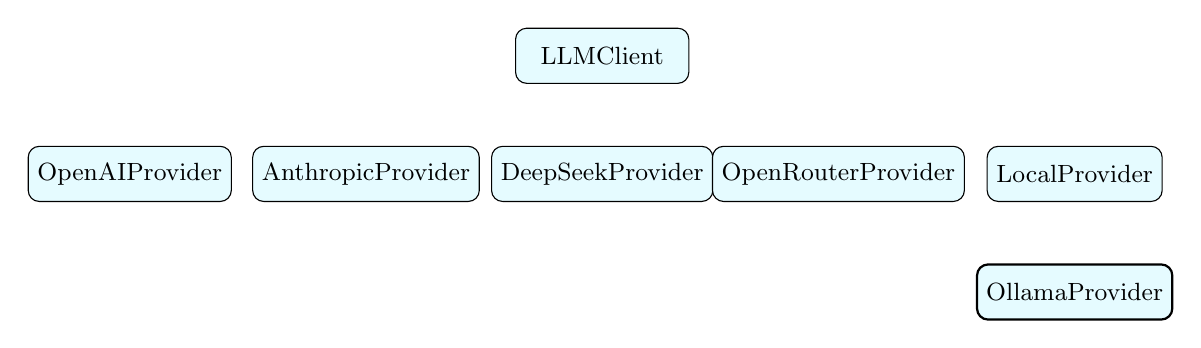
\begin{tikzpicture}[
    level distance=1.5cm,
    sibling distance=3cm,
    every node/.style={draw, rectangle, rounded corners, fill=phiblue!10, text centered, minimum width=2.2cm, minimum height=0.7cm, font=\small},
    edge from parent/.style={thick, ->, >=stealth}
]

    \node {LLMClient}
        child {node {OpenAIProvider}}
        child {node {AnthropicProvider}}
        child {node {DeepSeekProvider}}
        child {node {OpenRouterProvider}}
        child {node {LocalProvider}
            child {node {OllamaProvider}}
        };

\end{tikzpicture}
\caption{LLM Provider Hierarchy}
\label{fig:llm-providers}
\end{figure}

\subsection{Auto-Failover Priority Chain}

The LLM client builds a prioritized provider chain based on configured API keys:

\begin{enumerate}[leftmargin=*]
    \item \textbf{OpenAI} -- if \texttt{OPENAI\_API\_KEY} is set (models: gpt-4, gpt-4-turbo, gpt-3.5-turbo)
    \item \textbf{Anthropic} -- if \texttt{ANTHROPIC\_API\_KEY} is set (models: claude-3-opus, claude-3-sonnet, claude-3-haiku)
    \item \textbf{DeepSeek} -- if \texttt{DEEPSEEK\_API\_KEY} is set (uses OpenAI-compatible API)
    \item \textbf{OpenRouter} -- if \texttt{OPENROUTER\_API\_KEY} is set (gateway to 200+ models)
    \item \textbf{Local} -- if \texttt{LOCAL\_LLM\_URL} is set (llama.cpp, vLLM, etc.)
    \item \textbf{Ollama} -- if available at \texttt{http://localhost:11434}
\end{enumerate}

If one provider fails (rate limit, timeout, API error), the client automatically falls through to the next available provider in the chain.

\chapter{Perception Systems}

\section{Vision System}

\subsection{Architecture}

The Vision service (\texttt{backend/vision/}) provides real-time computer vision capabilities:

\begin{itemize}
    \item \textbf{Object Detection:} YOLOv8 nano for real-time object detection with configurable confidence threshold
    \item \textbf{Face Recognition:} face\_recognition library with known-face database
    \item \textbf{QR/Barcode Detection:} pyzbar library
    \item \textbf{Color Detection:} K-means clustering for dominant color extraction
    \item \textbf{Frame Capture:} Support for webcam, RTSP streams, and screen capture
\end{itemize}

\subsection{Data Flow}

\begin{figure}[H]
\centering
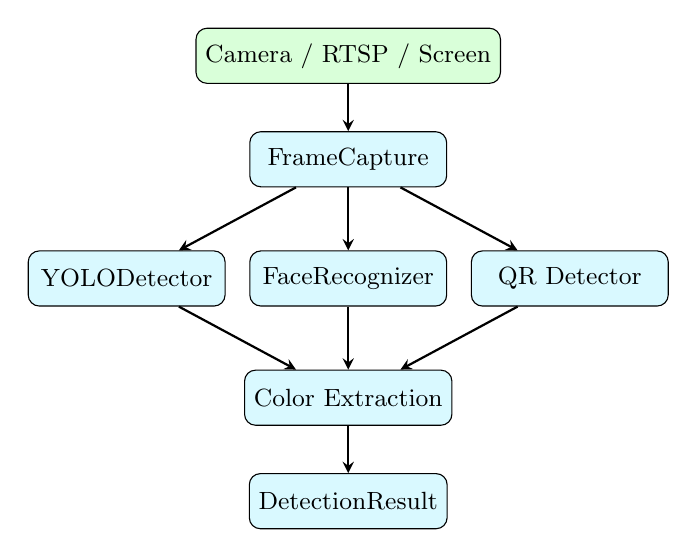
\begin{tikzpicture}[
    node distance=1.2cm,
    process/.style={rectangle, rounded corners, minimum width=2.5cm, minimum height=0.7cm, text centered, draw=black, fill=phiblue!15, font=\small},
    arrow/.style={thick, ->, >=stealth}
]

    \node[process, fill=green!15] (camera) {Camera / RTSP / Screen};
    \node[process, below=0.6cm of camera] (capture) {FrameCapture};
    \node[process, below left=0.8cm and 0.3cm of capture] (yolo) {YOLODetector};
    \node[process, below=0.8cm of capture] (face) {FaceRecognizer};
    \node[process, below right=0.8cm and 0.3cm of capture] (qr) {QR Detector};
    \node[process, below=0.8cm of face] (colors) {Color Extraction};
    \node[process, below=0.6cm of colors] (result) {DetectionResult};

    \draw[arrow] (camera) -- (capture);
    \draw[arrow] (capture) -- (yolo);
    \draw[arrow] (capture) -- (face);
    \draw[arrow] (capture) -- (qr);
    \draw[arrow] (yolo) -- (colors);
    \draw[arrow] (face) -- (colors);
    \draw[arrow] (qr) -- (colors);
    \draw[arrow] (colors) -- (result);

\end{tikzpicture}
\caption{Vision Data Flow}
\label{fig:vision-flow}
\end{figure}

\subsection{Detection Results}

\begin{table}[H]
\centering
\rowcolors{2}{gray!10}{white}
\begin{tabularx}{\textwidth}{|l|X|}
\hline
\rowcolor{phiblue!20}
\textbf{Field} & \textbf{Description} \\
\hline
objects & List of DetectedObject (label, confidence, bounding box, dominant color) \\
\hline
labels & All detected class labels \\
\hline
detection\_time\_ms & Inference time in milliseconds \\
\hline
frame\_width & Frame width in pixels \\
\hline
frame\_height & Frame height in pixels \\
\hline
dominant\_colors & RGB tuples from K-means clustering \\
\hline
\end{tabularx}
\caption{DetectionResult Fields}
\end{table}

\section{Hearing System}

\subsection{Architecture}

The Hearing service (\texttt{backend/hearing/}) handles audio capture and speech recognition:

\begin{itemize}
    \item \textbf{Microphone Capture:} PyAudio with background capture thread
    \item \textbf{Voice Activity Detection:} WebRTC VAD with configurable threshold and silence duration
    \item \textbf{Speech-to-Text:} OpenAI Whisper (local tiny model for speed, API for accuracy)
\item \textbf{Wake Word:} "Hey PHI" and "PHI" detection with
configurable sensitivity
    \item \textbf{Audio Ring Buffer:} Stores recent audio for context-aware processing
\end{itemize}

\subsection{Wake Word Processing Flow}

\begin{figure}[H]
\centering
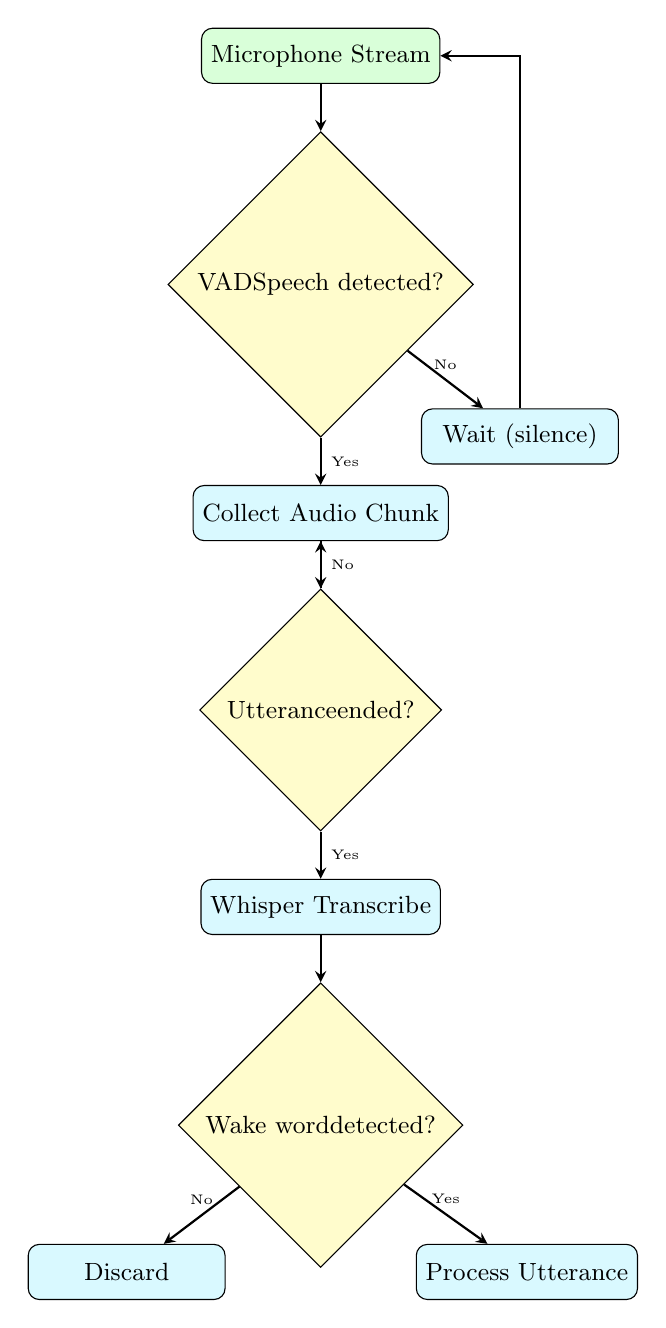
\begin{tikzpicture}[
    node distance=1.2cm,
    process/.style={rectangle, rounded corners, minimum width=2.5cm, minimum height=0.7cm, text centered, draw=black, fill=phiblue!15, font=\small},
    decision/.style={diamond, minimum width=1.8cm, minimum height=1.2cm, text centered, draw=black, fill=yellow!20, font=\small},
    arrow/.style={thick, ->, >=stealth}
]

    \node[process, fill=green!15] (mic) {Microphone Stream};
    \node[decision, below=0.6cm of mic] (vad) {VAD\\Speech detected?};
    \node[process, below right=0.6cm and 0.3cm of vad] (wait) {Wait (silence)};
    \node[process, below=0.6cm of vad] (buffer) {Collect Audio Chunk};
    \node[decision, below=0.6cm of buffer] (end) {Utterance\\ended?};
    \node[process, below=0.6cm of end] (transcribe) {Whisper Transcribe};
    \node[decision, below=0.6cm of transcribe] (wake) {Wake word\\detected?};
    \node[process, below left=0.6cm and 0.3cm of wake] (discard) {Discard};
    \node[process, below right=0.6cm and 0.3cm of wake] (process) {Process Utterance};

    \draw[arrow] (mic) -- (vad);
    \draw[arrow] (vad) -- node[above, font=\tiny] {No} (wait);
    \draw[arrow] (wait) |- (mic);
    \draw[arrow] (vad) -- node[right, font=\tiny] {Yes} (buffer);
    \draw[arrow] (buffer) -- (end);
    \draw[arrow] (end) -- node[right, font=\tiny] {No} (buffer);
    \draw[arrow] (end) -- node[right, font=\tiny] {Yes} (transcribe);
    \draw[arrow] (transcribe) -- (wake);
    \draw[arrow] (wake) -- node[above, font=\tiny] {No} (discard);
    \draw[arrow] (wake) -- node[above, font=\tiny] {Yes} (process);

\end{tikzpicture}
\caption{Wake Word Detection Flow}
\label{fig:wake-word}
\end{figure}

\section{Speech System}

\subsection{Architecture}

The Speech service (\texttt{backend/speech/}) provides text-to-speech synthesis with emotional expression:

\begin{itemize}
    \item \textbf{Primary Engine:} ElevenLabs API (highest quality, emotional range)
    \item \textbf{Fallback 1:} Coqui TTS (local open-source TTS)
    \item \textbf{Fallback 2:} gTTS (Google Text-to-Speech, last resort)
    \item \textbf{Emotional Support:} 8 emotions mapped to rate/pitch adjustments
    \item \textbf{Lip Sync:} Viseme generation for avatar mouth animation
    \item \textbf{Audio Effects:} Radio, echo, robotic, whisper, slow, fast
    \item \textbf{Caching:} LRU cache to avoid re-synthesizing common phrases
\end{itemize}

\subsection{Emotion Mapping}

\begin{table}[H]
\centering
\begin{tabularx}{\textwidth}{|l|X|l|l|}
\hline
\rowcolor{phiblue!20}
\textbf{Emotion} & \textbf{Effect} & \textbf{Rate Multiplier} & \textbf{Pitch Shift} \\
\hline
neutral & Standard speech & 1.0 & 0 \\
\hline
happy & Brighter, slightly faster & 1.15 & +1.5 \\
\hline
excited & Fast, high energy & 1.25 & +2.0 \\
\hline
serious & Slower, deeper & 0.85 & -2.0 \\
\hline
calm & Slow, soothing & 0.75 & -1.0 \\
\hline
angry & Faster, aggressive & 1.1 & -1.5 \\
\hline
sad & Slow, quiet, monotone & 0.7 & -2.5 \\
\hline
whisper & Quiet, breathy & 0.9 & -1.0 \\
\hline
\end{tabularx}
\caption{Emotion-to-Speech Parameters}
\end{table}

\subsection{TTS Synthesis Pipeline}

\begin{figure}[H]
\centering
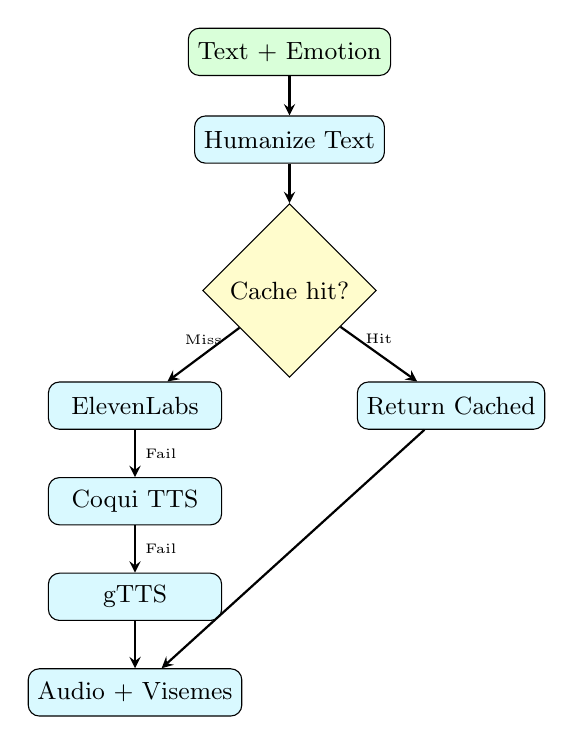
\begin{tikzpicture}[
    node distance=1cm,
    process/.style={rectangle, rounded corners, minimum width=2.2cm, minimum height=0.6cm, text centered, draw=black, fill=phiblue!15, font=\small},
    decision/.style={diamond, minimum width=1.5cm, minimum height=1cm, text centered, draw=black, fill=yellow!20, font=\small},
    arrow/.style={thick, ->, >=stealth}
]

    \node[process, fill=green!15] (input) {Text + Emotion};
    \node[process, below=0.5cm of input] (humanize) {Humanize Text};
    \node[decision, below=0.5cm of humanize] (cache) {Cache hit?};
    \node[process, below left=0.6cm and 0.3cm of cache] (eleven) {ElevenLabs};
    \node[process, below=0.6cm of eleven] (coqui) {Coqui TTS};
    \node[process, below=0.6cm of coqui] (gtts) {gTTS};
    \node[process, below right=0.6cm and 0.3cm of cache] (cached) {Return Cached};
    \node[process, below=0.6cm of gtts] (audio) {Audio + Visemes};

    \draw[arrow] (input) -- (humanize);
    \draw[arrow] (humanize) -- (cache);
    \draw[arrow] (cache) -- node[above, font=\tiny] {Miss} (eleven);
    \draw[arrow] (eleven) -- node[right, font=\tiny] {Fail} (coqui);
    \draw[arrow] (coqui) -- node[right, font=\tiny] {Fail} (gtts);
    \draw[arrow] (cache) -- node[above, font=\tiny] {Hit} (cached);
    \draw[arrow] (gtts) -- (audio);
    \draw[arrow] (cached) -- (audio);

\end{tikzpicture}
\caption{TTS Synthesis Pipeline with Fallback Chain}
\label{fig:tts-pipeline}
\end{figure}

\section{Action Service}

The Actions service (\texttt{backend/actions/}) provides executable capabilities:

\begin{table}[H]
\centering
\begin{tabularx}{\textwidth}{|l|X|}
\hline
\rowcolor{phiblue!20}
\textbf{Module} & \textbf{Capabilities} \\
\hline
api\_integrations.py & 16 API integrations: stocks, news, crypto, forex, sports, movies, music, nutrition, dictionary, jokes, quotes, holidays, IP geo, NASA, books, world time \\
\hline
file\_handler.py & Read/write CSV, Excel, PDF, JSON, YAML, XML, DOCX, PPTX, Markdown, SVG generation, LaTeX compilation \\
\hline
web\_scraper.py & Static HTML scraping, Playwright JS rendering, robots.txt compliance, article/product/table extraction \\
\hline
web\_search.py & SerpAPI, DuckDuckGo, OpenWeatherMap \\
\hline
email.py & SMTP email sending with HTML support \\
\hline
email\_reader.py & IMAP inbox reading with search \\
\hline
calendar.py & Google Calendar event creation \\
\hline
code\_sandbox.py & Isolated Python and JavaScript execution with timeout \\
\hline
database.py & SQLite, PostgreSQL, MySQL query execution \\
\hline
home\_assistant.py & MQTT smart home control (lights, temperature) \\
\hline
image\_gen.py & DALL-E 3 image generation \\
\hline
music.py & Spotify search, play, pause, current track \\
\hline
visualizations.py & Matplotlib charts: line, bar, pie, scatter, histogram, heatmap, 3D surface, animated charts \\
\hline
system\_commands.py & Open applications, take screenshots, system info \\
\hline
git\_ops.py & Git status, log, commit, push, pull, branch \\
\hline
document\_qa.py & Document ingestion and RAG-based Q\&A \\
\hline
notifications.py & Desktop and sound notifications \\
\hline
scheduler.py & In-memory task scheduling with reminders \\
\hline
avatar.py & Expression mapping, viseme shapes, head movement, body language \\
\hline
\end{tabularx}
\caption{Action Modules and Their Capabilities}
\end{table}

\chapter{Frontend Systems}

\section{React Application}

\subsection{Component Architecture}

The React frontend at \texttt{frontend/src/} is organized into six components:

\begin{figure}[H]
\centering
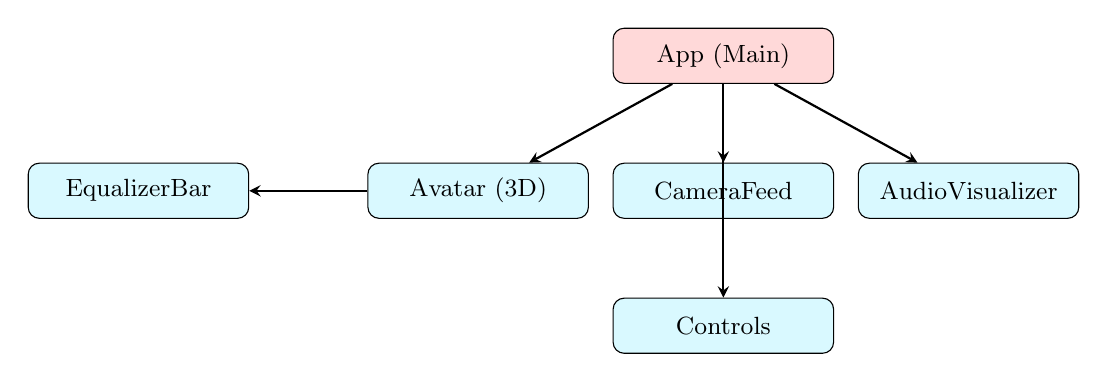
\begin{tikzpicture}[
    node distance=1.2cm,
    comp/.style={rectangle, rounded corners, minimum width=2.8cm, minimum height=0.7cm, text centered, draw=black, fill=phiblue!15, font=\small},
    arrow/.style={thick, ->, >=stealth}
]

    \node[comp, fill=red!15] (app) {App (Main)};
    \node[comp, below left=1cm and 0.3cm of app] (avatar) {Avatar (3D)};
    \node[comp, below=1cm of app] (camera) {CameraFeed};
    \node[comp, below right=1cm and 0.3cm of app] (audio) {AudioVisualizer};
    \node[comp, below=1cm of camera] (controls) {Controls};
    \node[comp, left=1.5cm of avatar] (eq) {EqualizerBar};

    \draw[arrow] (app) -- (avatar);
    \draw[arrow] (app) -- (camera);
    \draw[arrow] (app) -- (audio);
    \draw[arrow] (app) -- (controls);
    \draw[arrow] (avatar) -- (eq);

\end{tikzpicture}
\caption{React Component Hierarchy}
\label{fig:react-components}
\end{figure}

\begin{itemize}
    \item \textbf{App.js:} Main application with WebSocket manager, audio capture, state management, and three-panel layout
    \item \textbf{Avatar.js:} Three.js 3D avatar using react-three-fiber with MeshDistortMaterial, equalizer bars, and emotion-driven animation
    \item \textbf{CameraFeed.js:} getUserMedia-based camera capture with snapshot capability
    \item \textbf{AudioVisualizer.js:} Real-time 16-bar equalizer visualization
    \item \textbf{Controls.js:} Emotion override panel and command buttons
\end{itemize}

\subsection{WebSocket Integration}

The frontend maintains a persistent WebSocket connection to the orchestrator with auto-reconnect (3-second delay). Messages flow bidirectionally:

\begin{itemize}
    \item \textbf{Frontend $\rightarrow$ Backend:} Chat messages, audio chunks (base64), camera images (base64), commands
    \item \textbf{Backend $\rightarrow$ Frontend:} Chat replies, emotion updates, viseme frames, audio levels, listening status, mode changes
\end{itemize}

\subsection{State Management}

The App component maintains these state variables:

\begin{longtable}{|l|l|p{6cm}|}
\hline
\rowcolor{phiblue!20}
\textbf{State} & \textbf{Type} & \textbf{Description} \\
\hline
sessionId & string & Auto-generated session identifier \\
\hline
ws & WebSocket & Active WebSocket connection \\
\hline
messages & array & Chat message history \{role, text\} \\
\hline
inputText & string & Current text input value \\
\hline
isConnected & boolean & WebSocket connection status \\
\hline
emotion & string & Current emotion (neutral, happy, excited, etc.) \\
\hline
isSpeaking & boolean & PHI Agent is speaking \\
\hline
isListening & boolean & PHI Agent is listening \\
\hline
audioLevel & number & Current audio level (0-1) \\
\hline
visemes & array & Lip-sync frame data \\
\hline
equalizerData & array & 16-bin frequency data \\
\hline
micAvailable & boolean & Microphone accessibility \\
\hline
\end{longtable}
\caption{React Application State}

\section{3D Circular Equalizer}

\subsection{Architecture}

The standalone \texttt{equalizer.html} is a Three.js-powered 3D audio visualizer with 72 radial bars, beat detection, ADSR envelope, motion blur, particle systems, and WebSocket integration for automatic mode switching.

\subsection{State Machine}

The equalizer has four states driven by backend WebSocket mode events:

\begin{figure}[H]
\centering
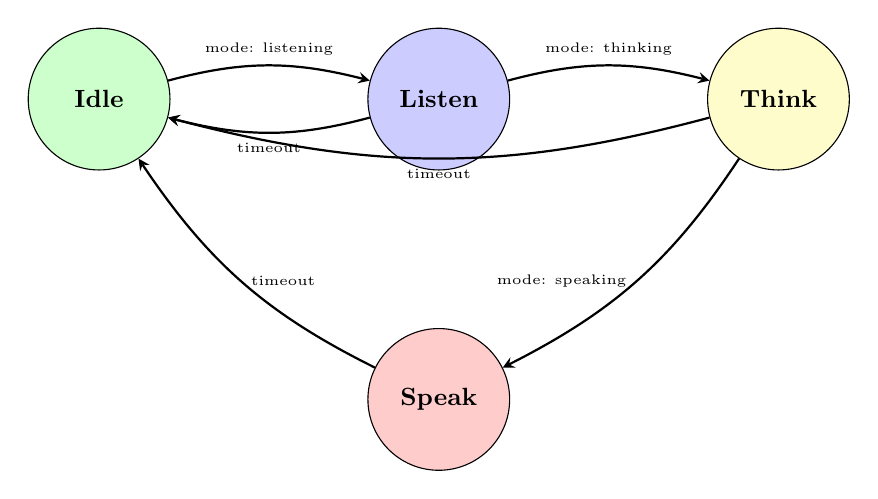
\begin{tikzpicture}[
    node distance=2cm,
    state/.style={circle, minimum width=1.8cm, text centered, draw=black, font=\small\bfseries},
    arrow/.style={thick, ->, >=stealth, bend left=20}
]

    \node[state, fill=green!20] (idle) {Idle};
    \node[state, fill=blue!20, right=2.5cm of idle] (listen) {Listen};
    \node[state, fill=yellow!20, right=2.5cm of listen] (think) {Think};
    \node[state, fill=red!20, below=2cm of listen] (speak) {Speak};

    \draw[arrow] (idle) to[bend left=15] node[above, font=\tiny] {mode: listening} (listen);
    \draw[arrow] (listen) to[bend left=15] node[above, font=\tiny] {mode: thinking} (think);
    \draw[arrow] (think) to[bend left=15] node[left, font=\tiny] {mode: speaking} (speak);
    \draw[arrow] (speak) to[bend left=15] node[right, font=\tiny] {timeout} (idle);
    \draw[arrow] (listen) to[bend left=15] node[below, font=\tiny] {timeout} (idle);
    \draw[arrow] (think) to[bend left=15] node[below, font=\tiny] {timeout} (idle);

\end{tikzpicture}
\caption{Equalizer State Machine}
\label{fig:eq-states}
\end{figure}

\subsection{EQ Profiles per Mode}

Each state has a unique EQ profile with gain offsets per frequency band, hue, and saturation:

\begin{table}[H]
\centering
\begin{tabularx}{\textwidth}{|l|X|l|l|l|l|l|l|}
\hline
\rowcolor{phiblue!20}
\textbf{State} & \textbf{Label} & \textbf{Low Bass} & \textbf{Bass} & \textbf{Mids} & \textbf{Presence} & \textbf{Treble} & \textbf{Hue} \\
\hline
Idle & CALM / STANDBY & +2 dB & +3 dB & 0 dB & -1 dB & -2 dB & 0.55 \\
\hline
Listen & LISTENING & 0 dB & 0 dB & +2 dB & +3 dB & -1 dB & 0.52 \\
\hline
Think & THINKING & 0 dB & 0 dB & 0 dB & 0 dB & 0 dB & 0.60 \\
\hline
Speak & SPEAKING & 0 dB & +2 dB & +2 dB & +4 dB & 0 dB & 0.48 \\
\hline
\end{tabularx}
\caption{EQ Profiles per Mode}
\end{table}

\subsection{Visual Components}

\begin{longtable}{|l|p{6cm}|l|}
\hline
\rowcolor{phiblue!20}
\textbf{Component} & \textbf{Description} & \textbf{Count} \\
\hline
Radial Bars & 72 bars arranged in circle with height driven by frequency + EQ gain + motion blur trails & 72 \\
\hline
Ambient Particles & Floating particles with color variation (blue, purple, pink) & 2800 \\
\hline
Trail Particles & Ghost particles for motion blur effect & 1500 \\
\hline
Particle Bursts & 2D canvas overlay bursts on beat detection & 200 max \\
\hline
Neon Rings & 3 decorative torus rings (outer, mid, inner) & 3 \\
\hline
Spin Rings & 2 rotating torus rings at different speeds & 2 \\
\hline
Core Orb & Central icosahedron sphere with wireframe overlay and floating torus & 3 meshes \\
\hline
Orbit Dots & 3 orbiting dots visible in THINK mode & 3 \\
\hline
Bass Rings & 2 torus rings that pulse with bass energy & 2 \\
\hline
Spectral History & Circular waterfall visualization (inner ring overlay) & 40 frames \\
\hline
Time-Domain Waveform & Circular waveform overlay (listen mode) & 200 samples \\
\hline
\end{longtable}
\caption{Equalizer Visual Components}

\subsection{Signal Processing Algorithms}

The equalizer implements 8 signal processing algorithms:

\begin{enumerate}[leftmargin=*]
    \item \textbf{Log-Scale FFT Mapping:} Perceptual frequency distribution using quadratic mapping: $\text{bin}_i = (\frac{i}{N})^2 \times \text{FFT\_size}$
    \item \textbf{Beat Detection:} Energy-based transient detector comparing instantaneous variance to historical variance with cooldown
    \item \textbf{ADSR Envelope:} Attack $t_a=0.08$, Decay $t_d=0.20$, Sustain $s=0.55$, Release $t_r=0.35$
    \item \textbf{Motion Blur Trails:} Ring buffer of 5 frames with exponential decay weighting ($w_t = e^{-t \times 0.6}$)
    \item \textbf{EQ Gain Scaling:} $\text{scale}(db) = 1.0 + db \times 0.04$
    \item \textbf{Transition Ramping:} easeInOutCubic smoothing over 200ms
    \item \textbf{HSL Color Mapping:} Hue from EQ profile + normalized amplitude ($\times 0.12$), saturation from profile, lightness $0.55 + \text{norm} \times 0.3$
    \item \textbf{Chromatic Aberration:} RGB emissive shift on core orb material with exponential decay ($\times 0.92$ per frame)
\end{enumerate}

\chapter{Configuration and Deployment}

\section{Configuration System}

\subsection{Environment Variables}

The configuration system (\texttt{backend/shared/config.py}) loads all settings from environment variables with sensible defaults:

\begin{longtable}{|l|l|l|}
\hline
\rowcolor{phiblue!20}
\textbf{Category} & \textbf{Variable} & \textbf{Default} \\
\hline
\multirow{4}{*}{Core} & USER\_NAME & User \\
 & PHI\_WAKE\_WORD & phi \\
 & LOG\_LEVEL & INFO \\
 & PHI\_DATA\_DIR & ./data \\
\hline
\multirow{4}{*}{API Keys} & OPENAI\_API\_KEY & (env) \\
 & ANTHROPIC\_API\_KEY & (env) \\
 & OPENROUTER\_API\_KEY & (env) \\
 & ELEVENLABS\_API\_KEY & (env) \\
\hline
\multirow{2}{*}{Redis} & REDIS\_HOST & localhost \\
 & REDIS\_PORT & 6379 \\
\hline
\multirow{3}{*}{ChromaDB} & CHROMA\_HOST & localhost \\
 & CHROMA\_PORT & 8000 \\
 & CHROMA\_COLLECTION & phi\_memory \\
\hline
\multirow{2}{*}{LLM} & LLM\_PROVIDER & openai \\
 & LLM\_MODEL & gpt-4 \\
\hline
\multirow{3}{*}{Memory} & MEMORY\_PALACE\_ENABLED & true \\
 & MEMORY\_PALACE\_ROOMS & 20 \\
 & MEMORY\_DIMENSION & 1536 \\
\hline
\multirow{3}{*}{Speech} & TTS\_ENGINE & elevenlabs \\
 & TTS\_VOICE\_ID & 21m00Tcm4TlvDq8ikWAM \\
 & TTS\_CACHE\_ENABLED & true \\
\hline
\multirow{3}{*}{Hearing} & WHISPER\_MODEL & tiny \\
 & VAD\_THRESHOLD & 0.5 \\
 & WAKE\_WORD\_SENSITIVITY & 0.5 \\
\hline
Services & ORCHESTRATOR\_PORT / VISION\_PORT / HEARING\_PORT / SPEECH\_PORT / ACTION\_PORT & 8000 / 8001 / 8002 / 8003 / 8004 \\
\hline
\end{longtable}
\caption{Key Configuration Environment Variables}

\section{Docker Deployment}

\subsection{Service Definitions}

\begin{table}[H]
\centering
\begin{tabularx}{\textwidth}{|l|l|l|X|}
\hline
\rowcolor{phiblue!20}
\textbf{Service} & \textbf{Image} & \textbf{Port} & \textbf{Depends On} \\
\hline
redis & redis:7-alpine & 6379 & --- \\
\hline
chroma & chromadb/chroma:latest & 8000 & --- \\
\hline
orchestrator & phi-backend & 8000 & redis, chroma \\
\hline
vision & phi-backend & 8001 & redis \\
\hline
hearing & phi-backend & 8002 & redis \\
\hline
speech & phi-backend & 8003 & redis \\
\hline
action & phi-backend & 8004 & redis \\
\hline
frontend & nginx:alpine & 3000:80 & orchestrator \\
\hline
\end{tabularx}
\caption{Docker Compose Services}
\end{table}

\subsection{Dockerfile Structure}

The backend runs on Python 3.11-slim with system dependencies (build-essential, ffmpeg, libsndfile1, libportaudio2), exposes ports 8000--8004, and starts via Uvicorn on port 8000.
\chapter{Data Models}

\section{Orchestrator Models}

All Pydantic models defined in \texttt{backend/orchestrator/models.py}:

\begin{table}[H]
\centering
\rowcolors{2}{gray!10}{white}
\begin{tabularx}{\textwidth}{|l|l|X|}
\hline
\rowcolor{phiblue!20}
\textbf{Model} & \textbf{Field} & \textbf{Description} \\
\hline
\multirow{5}{*}{ChatRequest} & message & User's text message \\
\cline{2-3}
 & session\_id & Session identifier (default: "default") \\
\cline{2-3}
 & emotion & Emotion hint (default: "neutral") \\
\cline{2-3}
 & image & Optional base64-encoded image \\
\cline{2-3}
 & context & Optional arbitrary context dictionary \\
\hline
\multirow{11}{*}{ChatResponse} & reply & Generated response text \\
\cline{2-3}
 & session\_id & Session identifier \\
\cline{2-3}
 & emotion & Detected emotion \\
\cline{2-3}
 & audio\_url & Optional TTS audio URL \\
\cline{2-3}
 & visemes & Optional lip-sync viseme sequence \\
\cline{2-3}
 & actions\_taken & List of executed tool names \\
\cline{2-3}
 & memory\_updated & Whether memory was modified \\
\cline{2-3}
 & processing\_time\_ms & Processing latency \\
\cline{2-3}
 & confidence & Response confidence score (0--1) \\
\cline{2-3}
 & intent & Classified intent \\
\cline{2-3}
 & tool\_recommendations & Suggested follow-up tools \\
\hline
\multirow{7}{*}{StatusResponse} & status & Service health ("ok", "degraded", "error") \\
\cline{2-3}
 & service & Service name \\
\cline{2-3}
 & version & Version string \\
\cline{2-3}
 & uptime\_seconds & Elapsed time since start \\
\cline{2-3}
 & active\_sessions & Concurrent session count \\
\cline{2-3}
 & memory\_status & Memory backend status \\
\cline{2-3}
 & services & Per-service health map \\
\hline
\multirow{5}{*}{WebSocketMessage} & type & Message type (chat, audio, video, command, emotion, viseme) \\
\cline{2-3}
 & payload & Arbitrary message payload \\
\cline{2-3}
 & session\_id & Session identifier \\
\cline{2-3}
 & timestamp & Unix timestamp of message \\
\hline
\end{tabularx}
\caption{Core Pydantic Models}
\end{table}

\section{Memory Models}

\begin{table}[H]
\centering
\rowcolors{2}{gray!10}{white}
\begin{tabularx}{\textwidth}{|l|l|X|}
\hline
\rowcolor{phiblue!20}
\textbf{Model} & \textbf{Field} & \textbf{Description} \\
\hline
\multirow{4}{*}{MemoryType (Enum)} & EPISODIC & Experiential memories (conversations, events) \\
\cline{2-3}
 & SEMANTIC & Factual knowledge (preferences, facts) \\
\cline{2-3}
 & PROCEDURAL & Skill/habit knowledge (routines, patterns) \\
\cline{2-3}
 & SPATIAL & Location-based memories (rooms, places) \\
\hline
\multirow{5}{*}{MemoryImportance (Enum)} & TRIVIAL & Minor casual mentions \\
\cline{2-3}
 & LOW & Minor facts \\
\cline{2-3}
 & NORMAL & Standard conversation summaries \\
\cline{2-3}
 & HIGH & Important information (preferences, key facts) \\
\cline{2-3}
 & CRITICAL & Essential data (passwords, configs) \\
\hline
\multirow{12}{*}{MemoryTrace} & id & Unique identifier \\
\cline{2-3}
 & content & Memory text content \\
\cline{2-3}
 & memory\_type & Type (Episodic/Semantic/Procedural/Spatial) \\
\cline{2-3}
 & importance & Importance level \\
\cline{2-3}
 & timestamp & Creation timestamp \\
\cline{2-3}
 & embedding & Vector embedding for similarity search \\
\cline{2-3}
 & metadata & Arbitrary key-value metadata \\
\cline{2-3}
 & room\_id & Assigned Memory Palace room \\
\cline{2-3}
 & access\_count & Retrieval frequency counter \\
\cline{2-3}
 & last\_accessed & Last access timestamp \\
\cline{2-3}
 & decay\_factor & Forgetting curve multiplier \\
\cline{2-3}
 & associations & Related memory IDs \\
\hline
\multirow{9}{*}{MemoryPalaceRoom} & id & Room identifier \\
\cline{2-3}
 & name & Room name (e.g. Library, Kitchen) \\
\cline{2-3}
 & description & Room purpose description \\
\cline{2-3}
 & topic & Domain topic \\
\cline{2-3}
 & emotional\_valence & Emotional tone of the room \\
\cline{2-3}
 & embedding & Room theme embedding \\
\cline{2-3}
 & created\_at & Creation timestamp \\
\cline{2-3}
 & memory\_ids & List of contained memory traces \\
\cline{2-3}
 & adjacent\_rooms & Related room connections \\
\hline
\end{tabularx}
\caption{Memory Data Models}
\end{table}

\section{Speech Models}

\begin{table}[H]
\centering
\rowcolors{2}{gray!10}{white}
\begin{tabularx}{\textwidth}{|l|l|X|}
\hline
\rowcolor{phiblue!20}
\textbf{Model} & \textbf{Field} & \textbf{Description} \\
\hline
\multirow{7}{*}{SynthesizeRequest} & text & Text to synthesize \\
\cline{2-3}
 & emotion & Emotion style (neutral, happy, excited, serious, calm, angry) \\
\cline{2-3}
 & return\_visemes & Whether to return viseme data for lip sync \\
\cline{2-3}
 & humanize & Apply natural speech patterns \\
\cline{2-3}
 & rate & Speech rate multiplier (0.5--2.0) \\
\cline{2-3}
 & pitch & Pitch shift in semitones \\
\cline{2-3}
 & effect & Audio effect (radio, echo, robotic, whisper, slow, fast) \\
\hline
\multirow{9}{*}{SynthesizeResponse} & audio & Base64-encoded audio data \\
\cline{2-3}
 & audio\_format & Format (wav, mp3, ogg) \\
\cline{2-3}
 & visemes & Lip sync viseme sequence (optional) \\
\cline{2-3}
 & emotion & Detected/applied emotion \\
\cline{2-3}
 & duration\_ms & Audio duration in milliseconds \\
\cline{2-3}
 & cache\_hit & Whether result was from cache \\
\cline{2-3}
 & latency\_ms & Processing latency \\
\cline{2-3}
 & rate & Applied speech rate \\
\cline{2-3}
 & pitch & Applied pitch shift \\
\hline
\end{tabularx}
\caption{TTS Request/Response Models}
\end{table}

\chapter{Extended Feature Modules}

\section{Color and Emotion Detection}

A comprehensive computer vision subsystem with 12 tools spanning color analysis and face-based emotion recognition. The color pipeline supports named-color mapping (28 named colors via Euclidean distance in RGB space), dominant color extraction via quantized bucket counting, monochromatic palette generation, and remote/local image analysis. The emotion pipeline integrates with DeepFace for face-based emotion/age/gender/race classification, OpenCV Haar Cascade for face detection, and BERT-based text emotion analysis with keyword fallback when transformers are unavailable.

\begin{figure}[H]
\centering
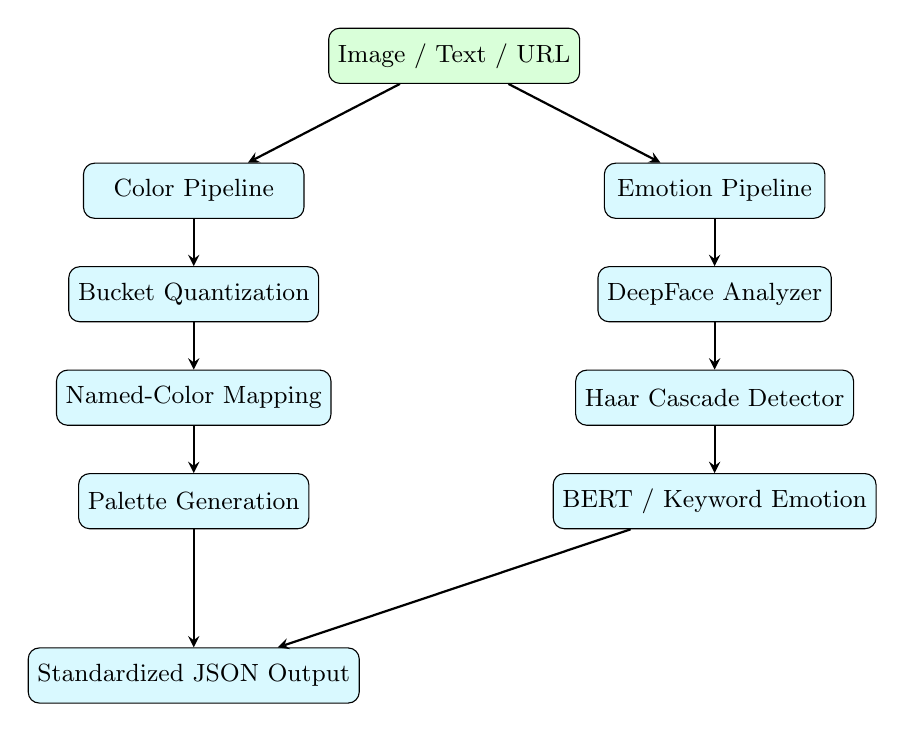
\begin{tikzpicture}[
    node distance=1.2cm,
    mod/.style={rectangle, rounded corners, minimum width=2.8cm, minimum height=0.7cm, text centered, draw=black, fill=phiblue!15, font=\small},
    arrow/.style={thick, ->, >=stealth}
]
    \node[mod, fill=green!15] (input) {Image / Text / URL};
    \node[mod, below left=1cm and 0.3cm of input] (color) {Color Pipeline};
    \node[mod, below right=1cm and 0.3cm of input] (emotion) {Emotion Pipeline};
    \node[mod, below=0.6cm of color] (bucket) {Bucket Quantization};
    \node[mod, below=0.6cm of bucket] (named) {Named-Color Mapping};
    \node[mod, below=0.6cm of named] (palette) {Palette Generation};
    \node[mod, below=0.6cm of emotion] (deepface) {DeepFace Analyzer};
    \node[mod, below=0.6cm of deepface] (haar) {Haar Cascade Detector};
    \node[mod, below=0.6cm of haar] (bert) {BERT / Keyword Emotion};
    \node[mod, below=1.5cm of palette] (output) {Standardized JSON Output};
    \draw[arrow] (input) -- (color);
    \draw[arrow] (input) -- (emotion);
    \draw[arrow] (color) -- (bucket);
    \draw[arrow] (bucket) -- (named);
    \draw[arrow] (named) -- (palette);
    \draw[arrow] (emotion) -- (deepface);
    \draw[arrow] (deepface) -- (haar);
    \draw[arrow] (haar) -- (bert);
    \draw[arrow] (palette) -- (output);
    \draw[arrow] (bert) -- (output);
\end{tikzpicture}
\caption{Color and Emotion Detection Pipeline}
\label{fig:color-emotion}
\end{figure}

\section{Shopping Assistant}

A full e-commerce assistant module with SQLite-backed product database, FAISS vector search for policy retrieval, and TF-IDF semantic routing. Stores 15 sample products across 6 categories with real-time search, recommendation scoring (weighted by price, rating, stock, and category match), and order tracking via a simulated state machine.

\begin{table}[H]
\centering
\rowcolors{2}{gray!10}{white}
\begin{tabularx}{\textwidth}{|l|X|}
\hline
\rowcolor{phiblue!20}
\textbf{Tool} & \textbf{Function} \\
\hline
product\_search\_db & Filtered product search by category, price range, rating \\
\hline
product\_get\_details & Full product details by ID \\
\hline
product\_list\_categories & Browsable category tree with product counts \\
\hline
policy\_search & Semantic policy lookup via FAISS embeddings \\
\hline
get\_product\_recommendations & Weighted recommendation scoring \\
\hline
check\_store\_policy & Return/exchange/shipping policy lookup \\
\hline
track\_order & Order status via simulated state machine \\
\hline
shopping\_route\_query & TF-IDF semantic router (product vs. general) \\
\hline
\end{tabularx}
\caption{Shopping Assistant Tools}
\end{table}

\section{Email and Calendar Agent}

A self-contained email management system with SQLite storage, vector-based semantic search, and calendar scheduling. Implements a Human-in-the-Loop (HITL) pattern for sensitive operations.

\begin{figure}[H]
\centering
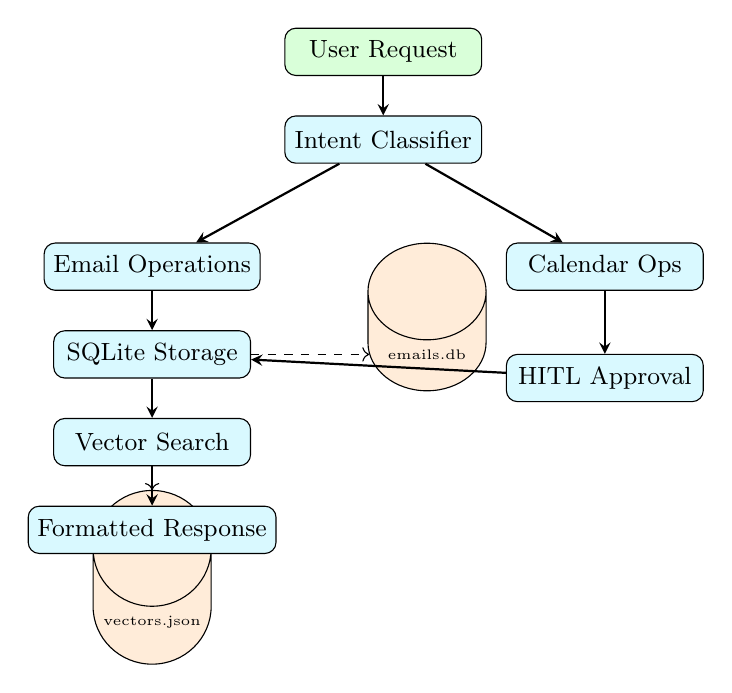
\begin{tikzpicture}[
    node distance=1cm,
    mod/.style={rectangle, rounded corners, minimum width=2.5cm, minimum height=0.6cm, text centered, draw=black, fill=phiblue!15, font=\small},
    db/.style={cylinder, shape border rotate=90, minimum width=1.5cm, minimum height=0.8cm, draw=black, fill=orange!15, font=\tiny},
    arrow/.style={thick, ->, >=stealth}
]
    \node[mod, fill=green!15] (input) {User Request};
    \node[mod, below=0.5cm of input] (classify) {Intent Classifier};
    \node[mod, below left=1cm and 0.3cm of classify] (email) {Email Operations};
    \node[mod, below right=1cm and 0.3cm of classify] (cal) {Calendar Ops};
    \node[mod, below=0.5cm of email] (sqlite) {SQLite Storage};
    \node[mod, below=0.5cm of sqlite] (vec) {Vector Search};
    \node[db, right=1.5cm of sqlite] (db) {emails.db};
    \node[db, below=0.3cm of vec] (vecidx) {vectors.json};
    \node[mod, below=0.8cm of cal] (hitl) {HITL Approval};
    \node[mod, below=0.5cm of vec] (resp) {Formatted Response};
    \draw[arrow] (input) -- (classify);
    \draw[arrow] (classify) -- (email);
    \draw[arrow] (classify) -- (cal);
    \draw[arrow] (email) -- (sqlite);
    \draw[arrow] (sqlite) -- (vec);
    \draw[arrow] (vec) -- (resp);
    \draw[arrow] (cal) -- (hitl);
    \draw[arrow] (hitl) -- (sqlite);
    \draw[->, dashed] (sqlite) -- (db);
    \draw[->, dashed] (vec) -- (vecidx);
\end{tikzpicture}
\caption{Email and Calendar Agent Architecture}
\label{fig:email-agent}
\end{figure}

\begin{longtable}{|l|X|}
\hline
\rowcolor{phiblue!20}
\textbf{Tool} & \textbf{Function} \\
\hline
\endhead
email\_search & Semantic + keyword email search over stored messages \\
\hline
email\_list\_inbox & List inbox/folder messages with pagination \\
\hline
email\_get\_message & Full message details (headers, body, attachments) \\
\hline
email\_send & Send email with CC support (HITL-gated) \\
\hline
email\_draft & Save draft without sending \\
\hline
email\_reply & Reply to a message thread \\
\hline
email\_mark\_read & Mark message as read \\
\hline
email\_star & Star/unstar a message \\
\hline
email\_archive & Archive a message \\
\hline
email\_trash & Move message to trash \\
\hline
email\_forward & Forward message with optional note \\
\hline
email\_search\_by\_sender & Filter messages by sender address \\
\hline
email\_get\_unread\_count & Quick unread badge count \\
\hline
email\_get\_attachment & Download attachment metadata \\
\hline
calendar\_list & List events for a date range \\
\hline
calendar\_create & Create event with attendees, location, duration (HITL-gated) \\
\hline
calendar\_update & Update event fields \\
\hline
calendar\_delete & Delete an event (HITL-gated) \\
\hline
calendar\_find\_slots & Find free time slots across schedule \\
\hline
\end{longtable}

\section{Data, Media, and Advanced Tool Libraries}

Three expanded tool modules adding 110+ utility functions covering data manipulation, media processing, and advanced text/security operations.

\subsection{Data Tools (35+ functions)}
String operations (reverse, upper, split, join, pad, truncate, replace, regex), list operations (shuffle, chunk, unique, flatten, zip, group, sort), dictionary operations (merge, flatten, pick, omit, sort\_keys, rename\_key), JSON operations (validate, diff, flatten, depth, merge, filter), math/statistics (mean, median, mode, stddev, correlation, percentile, factorial, gcd, lcm, fibonacci, prime\_check).

\subsection{Media Tools (30+ functions)}
Geographic utilities (distance, midpoint, bounding box, DMS conversion, elevation, timezone, sunrise/sunset), time utilities (now, epoch, diff, add, subtract, weekday, julian day, ISO format, age, leap year), file operations (copy, move, delete, rename, touch, size, modified), HTTP utilities (GET, POST, PUT, DELETE, PATCH with headers, download), format converters (JSON/YAML/XML/CSV/TOML/Markdown interconversion, HTML escape), encoding (base64, URL, slugify).

\subsection{Advanced Tools (45+ functions)}
Text intelligence (summarize, sentiment, keywords, readability, perplexity, plagiarism\_check, diff, detect\_language), security (hash\_text, encrypt/decrypt with Fernet, JWT token generation, password strength, port scan), development tools (uuid, ulid, cron\_next, cron\_describe, semver\_compare, diff\_patch), random generators (dice, lottery, tarot, zodiac, haiku, madlib, emoji, morse\_code, pig\_latin), format/unit converters (bytes, temperature, distance, weight, volume, speed, time, currency, number base, roman numeral).

\section{Understand-Anything Integration}

A complete knowledge graph generation pipeline that converts any codebase into an interactive, explorable architecture visualization. Uses a multi-agent pipeline with tree-sitter deterministic parsing for structural facts (imports, exports, definitions, call sites) and LLM-based semantic analysis for plain-English summaries, architectural layers, business domain mapping, and guided learning tours.

\begin{figure}[H]
\centering
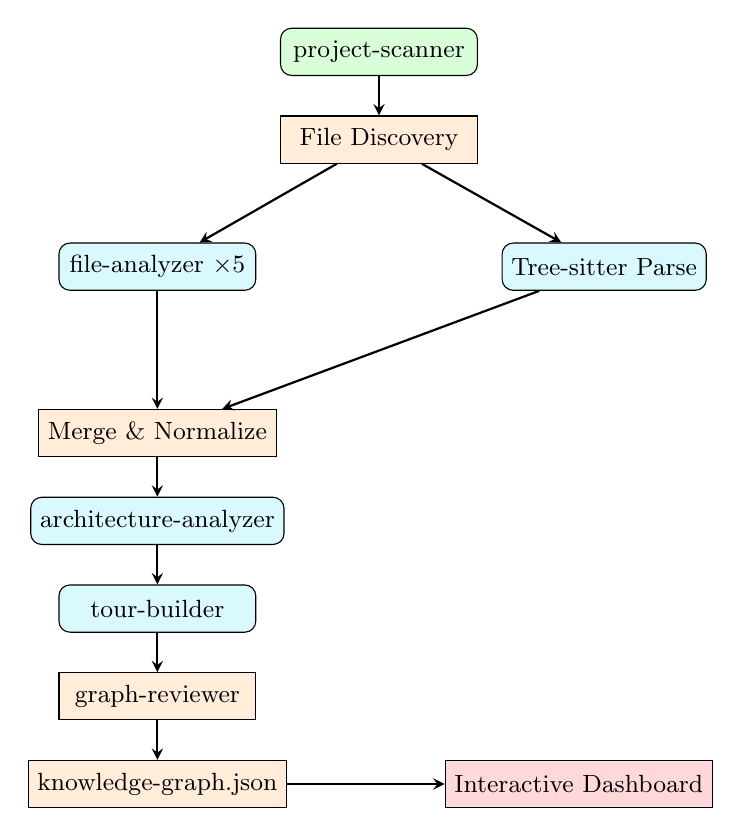
\begin{tikzpicture}[
    node distance=1.2cm,
    agent/.style={rectangle, rounded corners, minimum width=2.5cm, minimum height=0.6cm, text centered, draw=black, fill=phiblue!15, font=\small},
    stage/.style={rectangle, minimum width=2.5cm, minimum height=0.6cm, text centered, draw=black, fill=orange!15, font=\small},
    arrow/.style={thick, ->, >=stealth}
]
    \node[agent, fill=green!15] (scan) {project-scanner};
    \node[stage, below=0.5cm of scan] (files) {File Discovery};
    \node[agent, below left=1cm and 0.3cm of files] (fa) {file-analyzer $\times$5};
    \node[agent, below right=1cm and 0.3cm of files] (ts) {Tree-sitter Parse};
    \node[stage, below=1.5cm of fa] (merge) {Merge \& Normalize};
    \node[agent, below=0.5cm of merge] (arch) {architecture-analyzer};
    \node[agent, below=0.5cm of arch] (tour) {tour-builder};
    \node[stage, below=0.5cm of tour] (review) {graph-reviewer};
    \node[stage, below=0.5cm of review] (graph) {knowledge-graph.json};
    \node[stage, right=2cm of graph, fill=red!15] (dash) {Interactive Dashboard};
    \draw[arrow] (scan) -- (files);
    \draw[arrow] (files) -- (fa);
    \draw[arrow] (files) -- (ts);
    \draw[arrow] (fa) -- (merge);
    \draw[arrow] (ts) -- (merge);
    \draw[arrow] (merge) -- (arch);
    \draw[arrow] (arch) -- (tour);
    \draw[arrow] (tour) -- (review);
    \draw[arrow] (review) -- (graph);
    \draw[arrow] (graph) -- (dash);
\end{tikzpicture}
\caption{Understand-Anything Multi-Agent Pipeline}
\label{fig:understand-pipeline}
\end{figure}

Capabilities include:
\begin{itemize}[leftmargin=*]
    \item \textbf{/understand} -- Multi-agent codebase analysis producing a structured knowledge graph with 13 node types and 26 edge types
    \item \textbf{/understand-dashboard} -- Interactive web-based graph viewer with pan/zoom, fuzzy+semantic search, persona-adaptive UI
    \item \textbf{/understand-chat} -- Natural language querying over the codebase graph
    \item \textbf{/understand-diff} -- Git diff impact analysis showing affected components
    \item \textbf{/understand-explain} -- Deep-dive explanations of specific files, functions, or classes
    \item \textbf{/understand-domain} -- Business domain flow extraction (domains $\rightarrow$ processes $\rightarrow$ steps)
    \item \textbf{/understand-knowledge} -- Karpathy-pattern wiki analysis with entity extraction
    \item \textbf{/understand-onboard} -- Auto-generated team onboarding guides
\end{itemize}

\chapter{Roadmap}

\section{Feature Categories}

The project roadmap (\texttt{FEATURE\_ROADMAP\_200.md}) defines 362 items across 26 categories in 3 priority tiers:

\subsection{High Priority (Implement First)}

\begin{enumerate}[leftmargin=*]
    \item LLM \& AI Improvements (19 items)
    \item Memory \& Knowledge Base (10 items)
    \item Voice \& Audio (15 items)
    \item Avatar \& Expressions (10 items)
    \item Vision \& Computer Vision (8 items)
    \item Smart Home \& IoT (18 items)
    \item Calendar \& Scheduling (12 items)
    \item Email \& Communication (14 items)
    \item Web Search \& Info (14 items)
    \item Documentation \& Knowledge (8 items)
\end{enumerate}

\subsection{Medium Priority (Implement Next)}

\begin{enumerate}[leftmargin=*, start=11]
    \item File \& Data Management (16 items)
    \item Automation \& Workflows (22 items)
    \item Development \& Coding (18 items)
    \item Financial \& Analytics (22 items)
    \item Health \& Wellness (14 items)
    \item Entertainment \& Gaming (22 items)
    \item Travel \& Automotive (20 items)
    \item Shopping \& E-commerce (10 items)
\end{enumerate}

\subsection{Low Priority (Nice to Have)}

\begin{enumerate}[leftmargin=*, start=19]
    \item Learning \& Education (12 items)
    \item Art \& Creativity (10 items)
    \item Home, Garden \& Pets (18 items)
    \item Social \& Relationships (10 items)
    \item AI Agent Capabilities (13 items)
    \item Augmented Reality (8 items)
    \item Security \& Privacy (12 items)
    \item Notifications \& Alerts (8 items)
\end{enumerate}

\chapter{Appendix}

\section{Complete Tool List}

The full tool registry spans 300+ tools across 40+ categories. A condensed index is shown below; see the Tool Categories table in Section~\ref{sec:tool-categories} for the complete breakdown.

\begin{longtable}{|l|l|l|}
\hline
\rowcolor{phiblue!20}
\textbf{Tool Name} & \textbf{Category} & \textbf{Description} \\
\hline
\endhead
get\_time & utility & Current date and time \\
\hline
search\_web & information & Web search \\
\hline
get\_weather & information & Weather forecast \\
\hline
send\_email & communication & Send email \\
\hline
create\_calendar\_event & productivity & Create event \\
\hline
set\_reminder & productivity & Set reminder \\
\hline
control\_light & smart\_home & Smart light control \\
\hline
remember & memory & Store in long-term memory \\
\hline
recall & memory & Retrieve from memory \\
\hline
detect\_colors & vision & Dominant colors from camera \\
\hline
read\_file & filesystem & Read file contents \\
\hline
write\_file & filesystem & Write to file \\
\hline
read\_csv & data & Read CSV file \\
\hline
query\_json & data & Query JSON by key path \\
\hline
run\_python & development & Execute Python sandbox \\
\hline
get\_stock\_price & finance & Current stock price \\
\hline
convert\_currency & finance & Currency conversion \\
\hline
get\_joke & fun & Random joke \\
\hline
plot\_line\_chart & visualization & Line chart \\
\hline
extract\_dominant\_colors & vision & Dominant colors from image \\
\hline
color\_name\_from\_rgb & vision & Nearest named color \\
\hline
color\_palette\_generate & vision & Monochromatic palette \\
\hline
detect\_emotion\_face & vision & Face emotion (DeepFace) \\
\hline
detect\_emotion\_text & vision & Text emotion (BERT) \\
\hline
detect\_faces\_image & vision & Face detection (Haar) \\
\hline
analyze\_face\_attributes & vision & Age/gender/race/emotion \\
\hline
compare\_faces & vision & Face similarity \\
\hline
analyze\_emotion\_realtime & vision & Real-time emotion analysis \\
\hline
product\_search\_db & shopping & Product database search \\
\hline
policy\_search & shopping & Semantic policy lookup \\
\hline
track\_order & shopping & Order status \\
\hline
email\_search & email & Semantic email search \\
\hline
email\_send & email & Send email \\
\hline
calendar\_create & calendar & Create event \\
\hline
str\_reverse & data & String reversal \\
\hline
list\_shuffle & data & Shuffle list \\
\hline
dict\_merge & data & Merge dictionaries \\
\hline
stat\_mean & data & Statistical mean \\
\hline
geo\_distance & media & Geographic distance \\
\hline
time\_now & media & Current epoch time \\
\hline
file\_copy & media & Copy file \\
\hline
http\_get & media & HTTP GET request \\
\hline
json\_prettify & media & Pretty-print JSON \\
\hline
hash\_text & advanced & SHA-256 hash \\
\hline
encrypt\_text & advanced & Fernet encryption \\
\hline
summarize\_text & advanced & Text summarization \\
\hline
sentiment\_analysis & advanced & Sentiment score \\
\hline
generate\_password & security & Strong password \\
\hline
generate\_image & creative & DALL-E image generation \\
\hline
notify & system & Desktop notification \\
\hline
... (300+ total across 40+ categories) & & \\
\hline
\end{longtable}

\section{Requirements}

The project depends on a Python 3.12+ stack organized around FastAPI (async web framework), Redis (message broker), ChromaDB (vector database), and multiple AI/ML libraries:

\begin{table}[H]
\centering
\rowcolors{2}{gray!10}{white}
\begin{tabularx}{\textwidth}{|l|X|}
\hline
\rowcolor{phiblue!20}
\textbf{Category} & \textbf{Dependencies} \\
\hline
Web Framework & fastapi, uvicorn, pydantic, aiohttp, websockets, httpx \\
\hline
LLM Clients & openai, anthropic, tiktoken (OpenAI, Claude, DeepSeek, OpenRouter, Ollama, llama.cpp) \\
\hline
Database & chromadb, sentence-transformers, redis[hiredis], sqlite3 \\
\hline
Vision & opencv-python, ultralytics (YOLOv8), face-recognition, deepface, pyzbar \\
\hline
Audio & pyaudio, webrtcvad, openai-whisper, TTS (Coqui), gTTS \\
\hline
Data/ML & scikit-learn, pandas, numpy, matplotlib, scipy, transformers, torch \\
\hline
Utilities & pyautogui, paho-mqtt, spotipy, GitPython, apscheduler, python-dotenv, psutil \\
\hline
File Handling & openpyxl, PyMuPDF, python-docx, python-pptx, pyyaml \\
\hline
Security & cryptography, pyjwt, bcrypt \\
\hline
Testing & pytest, pytest-asyncio, pytest-cov \\
\hline
\end{tabularx}
\caption{Python Dependencies by Category}
\end{table}

\section{File Tree}

The updated project structure after cleanup:

\begin{longtable}{|l|X|}
\hline
\rowcolor{phiblue!20}
\textbf{Directory/File} & \textbf{Description} \\
\hline
\endhead
.env & Environment configuration \\
\hline
.env.example & Environment template \\
\hline
Dockerfile & Backend Docker image \\
\hline
opencode.json & opencode project configuration with skills.paths \\
\hline
README.md & Project overview \\
\hline
docker-compose.yml & Multi-service deployment \\
\hline
equalizer.html & Standalone 3D audio equalizer \\
\hline
requirements.txt & Python dependencies \\
\hline
start\_agent.py & CLI entry point \\
\hline
FEATURE\_ROADMAP\_200.md & 362-item roadmap \\
\hline
backend/orchestrator/ & FastAPI app, Pydantic models, agent + ToolRegistry \\
\hline
backend/memory/ & Memory Palace with 20 rooms (ChromaDB) \\
\hline
backend/speech/ & Multi-engine TTS, emotion mapping, lip sync \\
\hline
backend/hearing/ & PyAudio capture, VAD, Whisper STT \\
\hline
backend/vision/ & YOLOv8, face recognition, color/emotion detection \\
\hline
backend/actions/ & 30+ action modules (APIs, files, web, database, git, email, calendar, smart home, system, scheduler, shopping, etc.) \\
\hline
backend/tools/ & Autoregistered tool libraries: color\_emotion\_tools, data\_tools, media\_tools, advanced\_tools, shopping\_tools, email\_tools \\
\hline
backend/shared/ & Config, multi-LLM client, Redis client \\
\hline
frontend/ & React 18 + Three.js 3D avatar \\
\hline
docs/ & API reference, deployment guide, this .tex doc \\
\hline
scripts/ & CLI tool \\
\hline
locale/ & Internationalization \\
\hline
.understand-anything/ & Understand-Anything scan results, batches, .understandignore \\
\hline
\end{longtable}

\end{document}
